% 学号
% !Mode:: "TeX:UTF-8"
% !TEX builder = LATEXMK
% !TEX program = xelatex
\documentclass[oneside,nocpsupervisor]{zjuthesis}

%\documentclass[doctor,twoside,nocpsupervisor]{zjuthesis}
\usepackage{color}
\usepackage{multirow}
\usepackage[scientific-notation=true,round-precision=4,round-mode=figures]{siunitx}

% 插图路径设置,图片放在figures 文件夹下。一般来说论文的插图比较多,通常按章节存
% 放,因此可以在以下命令中在按章节添加存放图片的文件夹路径。如以下这个路径中 ./
% 代表当前main.tex所在的目录,就是一般所说的当前文件夹;figures 文件夹就是子文件
% 夹,存放正文及附录中要用到的所有的图片,在figures 文件夹中的子文件夹就是存放各
% 个章节图片的文件夹,一般命名与相应章节的名字相同,如intro 章节用到的图片全放在
% 了intro 这个子文件夹下。
\graphicspath{%
	{./figures/intro/}%
	{./figures/sffd/}%
	{./figures/clip/}%
	{./figures/gpu/}%
	{./figures/mobile/}%
	{./figures/result/}%
}

% 论文中文标题
\title{改进的光滑自由变形及其应用}
% 论文英文标题
\englishtitle{Improved Smooth Free-Form Deformation}
% 作者,就是你的名字
\author{陆哲琪}
% 分类号
\classification{TM863}
% 单位代码
\serialnumber{10335}
% 密级
\secretlevel{公开}
% 学号
\studentnumber{21421007}
% 指导教师
\supervisor{冯结青}
% 合作导师,如果没有合作导师,就在\documentclass选项栏中加上"nocpsupervisor"。
\cpsupervisor{冯结青}
% 专业名称
\major{计算机技术}
% 研究方向
\research{图形学方向}
% 所在学院
\institute{计算机学院}
% 提交日期
\submitdate{2017年1月5日}

% 中文题名页
\reviewerA{关羽\hspace{1.5em}五虎上将\hspace{1.5em}蜀汉}
\reviewerB{张飞\hspace{1.5em}五虎上将\hspace{1.5em}蜀汉}
\reviewerC{马超\hspace{1.5em}五虎上将\hspace{1.5em}蜀汉}
\chairperson{许攸\hspace{1.5em}文臣谋士\hspace{1.5em}曹魏}
\commissionerA{法正\hspace{1.5em}文臣谋士\hspace{1.5em}蜀汉}
\commissionerB{简雍\hspace{1.5em}文臣谋士\hspace{1.5em}蜀汉}
\commissionerC{麋竺\hspace{1.5em}文臣谋士\hspace{1.5em}蜀汉}
\defencedate{2017年3月5日}

\begin{document}
\maketitle
% \ZJUmakecover
% \ZJUmakeCNtitlepage
% \ZJUmakeENtitlepage
\frontmatter
% !TEX root = ../main.tex

% 定义中文摘要和关键字
\begin{cabstract}
    自由变形\cite{Sederberg86}(Free Form Deformation,简称FFD)是一类编辑几何模型、生成柔体性动画的方法。由于其实现简单,与模型表示无关,所以被广泛的应用于计算机辅助设计与工程、计算机动画、医学影影等领域。另一方面,由于其较强的可拓展性,FFD\cite{Sederberg86}自提出以来就受到了学术届与工业界的广泛关注,该工作不仅实现了一种具体的编辑三维模型的方法,更重要的是提出了一套编辑三维模型的算法框架。

在该框架基础上,研究人员提出了许多方法以改进原有的FFD的一些不足之处,如变形结果走样,交互繁琐,效率低下等问题。

    崔的光滑自由变形\cite{Cui15}也是基于FFD框架的一种空间变形算法,主要在算法效率、变形结果质量这两方面对前人的工作作出了改进。使得用户可以实时的编辑三维模型,且能得到光滑细腻的变形。

    但其仍存在一些问题:1)算法在预处理阶段,会沿变形空间的结点盒对待变形模型形进行裁剪。但是裁剪可能会产生狭长多边形甚至退化多边形,这些多边形不仅会浪费计算资源,还会带来精度和程序鲁棒性的问题。2)光滑自由变形使用了CUDA做并行计算,以保证变形算法的实时性,但是CUDA只能在Nvidia的平台止运行,这大限制了光滑自由变形的通用性。

    因此,本文提出了一种基于光滑自由变形的新的变形算法,针对上述问题做出了相应的改进。

    首先,本文提出了一种新的多边形裁剪算法----三角均匀剖分算法。该算法以任意三角形为输入,对三角形进行分割,使产生的子三角形的形状尽可能接近正三角形且面积尽可能相等。此处,本文还对新旧两种分割算法进行了比较,并探索了新的分割算法对变形质量,运行效率的影响。

    其次,本文用OpenGL的Compute Shader实现了本文算法中除初始化之外的所有部分,在保证算法通用性的同时,尽可能地提高了算法的计算效率。同时,为了验证本文算法在不同平台下的通用性以及算法在计算资源较匮乏的情境下的表现,我们还在一个安卓平台的应用中实现了本文算法。

    最后,我们将本文算法与精确自由变形、光滑自由变形等方法进行多方面的对比。以体现本文方法的优势。
\end{cabstract}

\ckeywords{光滑自由变形,保留尖锐特征,OpenGL 计算着色器,图形处理单元,法向量场,三角形均匀剖分}

% !TEX root = ../main.tex

% 定义英文摘要和关键字

\begin{eabstract}
    Free-form deformation\cite{Sederberg86}(FFD) is a prevalent shape manipulation and shape animation method in computer graphics and geometric modeling. It is widely used in Computer-aided Design, Computer Animation, Medical Imaging and so on. However, there are some disadvantages in the FFD, such as the aliasing of deformation result, universality and robustness, low efficiency and so on. In order to address these problems, we propose the Improved Smooth Free-form Deformation.

    Our method will be used to clip the original model to avoid pathological case. Our subdivision method will produce sub-triangles as regular as possible, but cannot guarantee that each sub-triangle lies in a knot box. Accordingly the method will introduce acceptable errors. However, the trade-off is worthwhile in accordance with Error analysis. 

    Moreover, we implement the whole framework of Improved Smooth FFD with OpenGL compute shader in order to make it more general. We also extend the deformation framework to the mobile phone by the aid of the across-platform of OpenGL.

    Finally, we contrast our method with the Smooth FFD and Accurrate FFD to show the advantage of our method.
\end{eabstract}

\ekeywords{smooth FFD, sharp feature preserving, GPU, OpenGL compute shader, normal field}

% 正文目录:
\tableofcontents
% 插图目录:
\listoffigures
% 表格目录:
\listoftables
% !TEX root = ../main.tex
\begin{denotation}

\item[GPU] 图形处理器 (Graphics Processing Unit)
\item[FFD] 自由变形 (Free Form Deformation)
\item[GPGPU] 通用计算 (General-purpose computing on graphics processing units)
\item[VR] 虚拟现实 (Virtual Reality)
\item[AR] 增强现实 (Augmented Reality)
\item[CVT] Centroidal Voronoi tessellation
\item[CUDA] 统一计算架构(Compute Unified Device Architecture)
\item[API] 应用程序接口(Application Programming Interface)
\item[AMD] 超威半导体(Advanced Micro Devices)



\end{denotation}

\mainmatter
% !TEX root = ../main.tex

\chapter{绪论}
\section{引言}
三维模型形状编辑是图形学及其相关领域中不可或缺的一部分。其无论在研究还是工业领域都存在着广泛的需求。研究人员提出了很多方法以满足不同场景下的编辑需求。其中,空间变形是一种出现时间比较早,应用比较广泛的模型形状编辑算法框架。该方案的基本思想最初由Barr\cite{Barr84}在1984年提出。Sederberg\cite{Sederberg86}于1986提出了经典的自由变形(Free-Form Deformation, 简称FFD),将这一思想完善为一个成熟的算法框架:
\begin{enumerate}
	\item 定义一个变形空间,也可以称之为中间体。
    \item 将待变形的模型“嵌入”到变形空间中,即计算模型上的采样点在变形空间中的参数坐标,该坐标在变形过程中保持不变。\label{item:2}
	\item 对变形空间进行变形。\label{item:3}
    \item 根据\ref{item:2}中得到的参数坐标与\ref{item:3}中得到的新变形空间,重新计算出采样点在欧氏空间中的坐标,从而达到变形的目的。
\end{enumerate}

该方法具有直观、简单、高效的优点,很多学者在在此基础上提出了大量关于FFD算法的研究与改进。

中间体的选取是空间变形算法的关键,算法的效率、交互方式、变形结果等会因中间体表达方式的改变而改变。所以很多研究工作都着眼于中间体的改进:

Griessmair\cite{Griessmair89}和Lamousin\cite{lamousin1994}分别用B样条体和非均匀有理B样条体替换传统FFD\cite{Sederberg86}中的贝赛尔体,由于B样条体和非均匀有理B样条体的局部支撑性,使得模型的变形具有局部可调性。Coquillart\cite{coquillart1990}则通过移动、“焊接”长方体控制网格中的部分控制顶点,使得控制网格不再局限于长方体,而是将其转变圆柱等更加复杂的形状。这一改变虽然增加了变形模型嵌入变形空间过程中的计算量且对于控制网格的形状有一定的限制,但是改进了交互方式,使用户能够进行更为复杂的变形。

后续的学者进一步提出了以曲面、曲线甚至是以点为变形工具来构建变形空间。这些方法各自适用于不同的变形场合。如基于曲线的FFD适合基于骨架变形或者细长物体的变形,基于曲面的变形比较适用于形状较为扁平的模型的变形。总体而言,用户编辑模型时可以控制的变量越多,算法对模型的编辑能力就越强,能完成更加复杂的变形,但同时用户的交互也越复杂。在Gain和Beckmann的综述\cite{Gain08}中,作者对常见的FFD按照选用变形空间的不同进行了分类,并从局部可调性、交互友好度、时空效率、是否保拓扑等方面详细对比了各个方法的优劣。

上述这些方法中,无论中间体如何选择,用户都需要通过操作控制顶点来对中间体进行变形,中间体再通过采样点的参数坐标将变形“传导”到待变形的模型中。这一交互方式对普通用户而言并不友好,控制顶点的位移与待变形模型的顶点的位移并不完全一致。用户需对中间体的数学表示有所了解,才能实现复杂的变形意图。

为了解决这一问题,Hsu\cite{hsu1992}最先提出了直接自由变形,这一算法允许用户指定待变形模型上的一组点,并由用户提供这组点变形前后在欧氏空间中的位移。以前述信息为输入,算法将自动求出一组合适的控制顶点,使得用户指定的点的位移与输入保持一致。再由这组控制顶点求得最终变形结果。

随后,其它研究者也在此基础上提出了许多类似方法。这一类方法直接关联用户输入和变形结果,使用户直接编辑模型变形前后关键点的位置,即可等到整体的变形结果,而无需关心中间体的数学表示。使得FFD的交互更加便捷、直观。

传统FFD方法的另一个不足之处是变形过程中的走样问题。

由于传统FFd方法将变形是作用到待编辑模型的采样点上的,再由采样点变形后的位置,还原出模型的变形结果。所以,最终得到的变形结果的质量很大程度上依赖于采样点的密度。下\autoref{fig:sample_problem}很好的演示了这一问题。柜子的四个腿在原模型中由狭长的三角形组成,并且从视觉上看是与底部十字木条连在一起的。但是若以模型顶点为采样点,进行如\autoref{subfig:sample_problem_1}所示的变形后,柜子腿从视觉上与底部的十字木条分开了。这是由于采样点过于稀疏,变形只作用于柜子腿底部的顶点,而未作用于柜子腿与十字木条相连的部分造成的。

\begin{figure}[htbp]
	\centering
	\begin{subfigure}[b]{.4\textwidth}
		\centering
		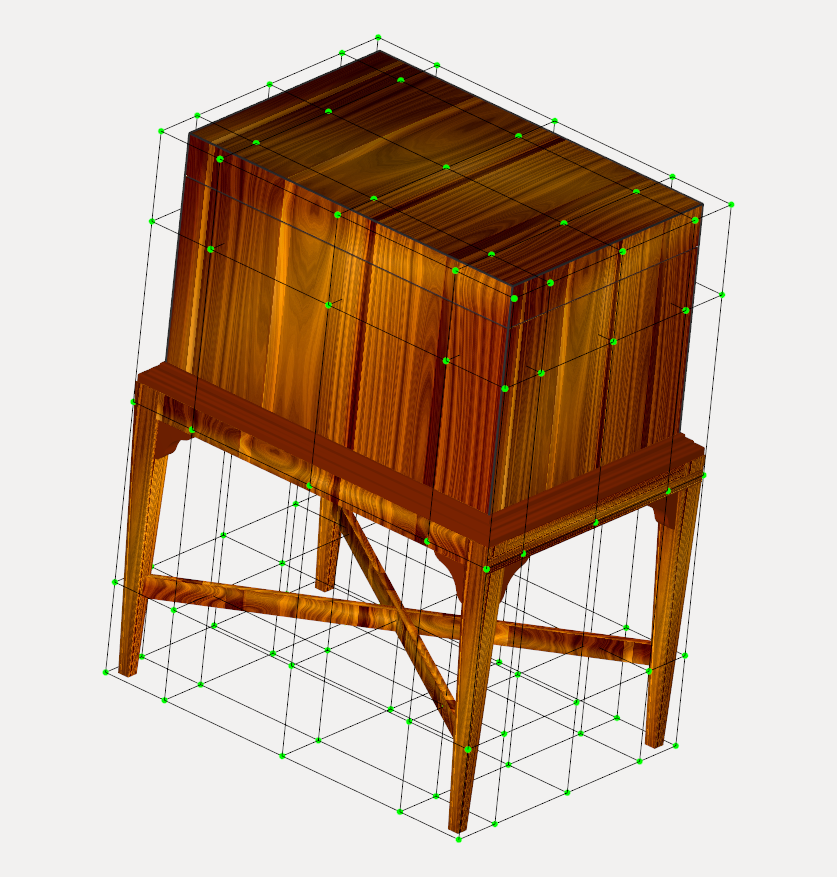
\includegraphics[width = \textwidth]{sample_problem_1.png}
		\caption{原模型}\label{subfig:sample_problem_0}
	\end{subfigure}
	\quad
	\begin{subfigure}[b]{.4\textwidth}
		\centering
		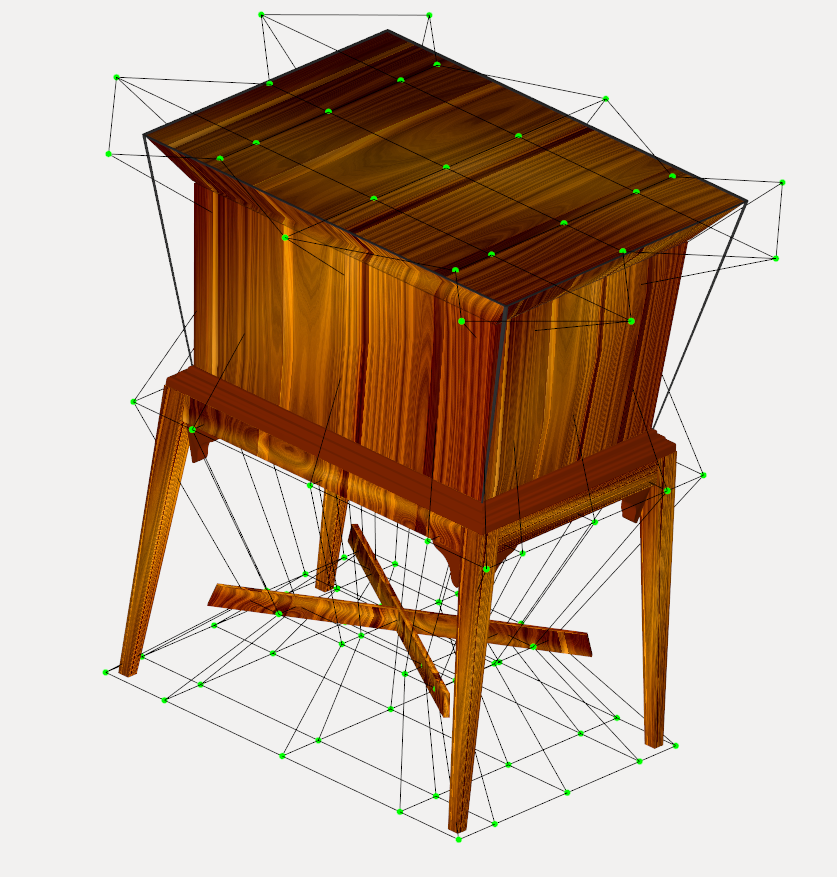
\includegraphics[width = \textwidth]{sample_problem_2.png}
		\caption{传统FFD变形结果}\label{subfig:sample_problem_1}
	\end{subfigure}
    \caption{传统FFD由于采样密度不足造成的精度问题}\label{fig:sample_problem}
\end{figure}

这一问题最直接的解决办法是通过均匀加密采样增加采样点的密度,但这一方法会造成性能上较大的开销。更进一步的方法\cite{parry1986, gain1999}是根据面片大小和曲面的曲率,自适应确定采样密度.自
适应采样虽然从性能上较之均匀加密采样有了较大的提升,但是其实现相对复杂,并且无法很好的处理一些奇异情况。

造成采样问题的根本原因是用







%自由变形(Free Form Deformation)是一类编辑几何模型、生成柔体性动画的方法。由于其实现简单,与模型表示无关,所以被广泛的应用于计算机辅助设计与工程、计算机动画、医学景象等领域。另一方面,由于其较强的可拓展性,FFD\cite{Sederberg86}自提出以来就受到了学术届的广泛关注,该工作不仅实现了一种具体的编辑三维模型的方法,更重要的是是提出了一套编辑三维模型的算法框架。研究人员在这一框架的基础上,做了很多工作。主要从算法效率、变形结果、交互方式三方面对FFD进行了改进:

%FFD的构架下的算法大多是计算密集形的,所以在很难做到实时交互。但因为这些算法能较好的适用于单指令流多数据流计算模型,所以随着通用计算的兴起,很多学者采用GPU加速这些算法,使其效率得到了较大的提升,从而使该方法能对大型三维模型进行实时编辑。



%在FFD交互方式的探索中,研究者主要着眼于变形空间的选取。不同的变形空间,适用于不同的编辑需求,同时也会影响用户的交互方式。总体而言,用户编辑模型时可以控制的变量越多,算法对模型的编辑能力就越强,同时用户的交互也越复杂。

\section{相关工作}

\section{本文内容安排}

\section{引言}
以下是一个测试用的列表环境,内容不要在意。\footnote{正文中中脚注命令测试,长脚注情况:这包括如下事实:“未经本人同意,监听、录制或转播私人性质的谈话或秘密谈话;未经本人同意,拍摄、录制或转播个人在私人场所的形象”}

这里测试列表标签功能的交叉引用格式\ref{itm:11},\ref{itm:12},\ref{itm:13},\ref{itm:14},分别表示第一至第四层级的itemize系列的交叉引用情况。
\begin{enumerate}
	\item 第一级列表\label{itm:11}
	\item 第一级列表
	\begin{enumerate}
		\item 第二级列表\label{itm:12}
		\item 第二级列表
		\begin{enumerate}
			\item 第三级列表\label{itm:13}
			\item 第三级列表
			\begin{enumerate}
				\item 第四级列表\label{itm:14}
				\item 第四级列表
				\item 第四级列表
				\item 第四级列表
			\end{enumerate}
			\item 第三级列表
			\item 第三级列表
			\item 第三级列表
		\end{enumerate}
		\item 第二级列表
		\item 第二级列表
	\end{enumerate}
	\item 第一级列表
	\item 第一级列表
	\item 第一级列表
\end{enumerate}

正是由于油膜物质的发现,使“雾伞”计划成为可能,这个计划是用核爆炸在太空中蒸发和扩散油膜物质,在太阳与地球之间形成一团“油膜尘埃”,降低太阳 对地球的辐射,达到缓解地球温室效应的目的。“我记得,海王星轨道附近应该还有前战争时期的恒星型核弹吧?”肯又问。“有的,‘雾伞’工程的飞船也装载了一些,在海王星环和卫星上爆破用,具体数目不清楚。” “好像一颗就够了。”肯兴奋起来。两个世纪前面壁者雷迪亚兹的战略计划中所研制的恒星型氢弹,后来共制造了五千多颗。虽然这种武器在末日之战中作用有限,但正如雷迪亚兹所言,各大 国主要是为可能爆发的人类之间的行星际战争准备的,核弹主要在大低谷时期制造,那时由于资源的匮乏,国际关系极其紧张,人类自身的战争一触即发。进入新时期后,这些骇人听闻的武器成了危险的鸡肋,虽然其所有权都属于地球国家, 但还是都被送入太空存贮,少部分已经用于行星工程的爆破,还有一部分送入太阳系外围轨道。曾有人设想将核弹中的聚变材料可以作为远程飞船的燃料补充,但由于核弹的拆解很困难,这个设想一直没有真正实现过\footnote{看看另起一页脚注编号的变化}。
\begin{itemize}
	\item 第一级列表
	\item 第一级列表
	\begin{itemize}
		\item 第二级列表
		\item 第二级列表
		\begin{itemize}
			\item 第三级列表
			\item 第三级列表
			\begin{itemize}
				\item 第四级列表
				\item 第四级列表
				\item 第四级列表
				\item 第四级列表
			\end{itemize}
			\item 第三级列表
			\item 第三级列表
			\item 第三级列表
		\end{itemize}
		\item 第二级列表
		\item 第二级列表
	\end{itemize}
	\item 第一级列表
	\item 第一级列表
	\item 第一级列表
\end{itemize}

“你觉得能行,”罗宾逊两眼放光地问道,他后悔这么简单的事自己怎么没 想到,一个载入史册的机会让肯抢去了。“试试吧,只有这一个办法了。”“如果行,博士,以后林格一斐兹罗监测站将永远按产生1G重力的速度旋转。”“这可是人类造出来的最大的东西了。”“蓝影”号飞船的指令长看着舱外漆黑的太空说,他极力想象自己能看到尘埃云,但确实什么\footnote{连续两个脚注测试1}\footnote{连续两个脚注测试2}
\begin{enumerate}
	\item 第四级列表
	\item 第四级列表
	\begin{enumerate}
		\item 第五级列表
		\item 第五级列表
		\item 第五级列表
	\end{enumerate}
	\item 第四级列表
	\item 第四级列表
\end{enumerate}
都看不到。“为什么它不能被阳光照出来呢,就像彗星的尾巴那样...”飞船驾驶员说,“蓝影”号上只有他和指令长两个人。他知道,尘埃云的密度确实像彗星尾一样稀薄,几乎和地球上实验室中造出的真空差不多。“可能是阳光太弱吧。”指令长回头看看太阳,在这海王星轨道和柯伊伯带 之间的冷寂空间,太阳看上去只是一颗刚能看出圆盘形状的大星星。阳光倒是还可以在舱壁上照出亮影,但已经十分微弱了。“再说,彗尾也要在一定的距离外 才能看到,我们可是就在云的边缘。”

\section{相关工作}
测试一下引用\cite{shi_chinas_2010},引用\cite{shi2010china,hata2014soi,muhammad2011development},还有其它引用\cite{shi2010china,muhammad2011development,lamport1994latex}.

\section{浮动体测试}
\subsection{插图测试}
如\autoref{fig:first_image_tset}是对此模版的第一张插图测试。

\begin{figure}[htbp]
	\centering
	
\includegraphics[width = 0.5\linewidth]{Chapter1.png}
	\caption{第一张插图测试}\label{fig:first_image_tset}
\end{figure}

以下是一段对这些插图来历的介绍,引用自知乎专栏All about TeXnique中夏晓昊的文章\href{http://zhuanlan.zhihu.com/LaTeX/19669122}{《The TeXbook导读:从那头(多图杀猫的)狮子说起》}。

在The TeXbook中,有着一系列的以狮子为主题的插图。这些插图的作者是Duane Bibby。也是从The TeXbook开始,不少TeX书也采取了以狮子为主的插图,作者也是Duane Bibby。另外,每年的TUG(TeX Users Group)年会都会有一张以狮子为主题的logo,这只狮子已经是社区的吉祥物了。

为什么选择狮子呢?Yannis Haralambous写道(原文法语,此为转译后的英文):Not for nothing is TeX represented by a lion. Donald Knuth has told us that lions are to him the guardians of libraries in the United States because there is a statue of a lion in front of the entrance of each large library there. Guardian of libraries, guardian of the Book—is that not indeed what TeX ultimately aspires to be? 或许吧。 (顺便说一句,TeX和MetaFont都用了狮子,TeX是公狮子,MetaFont是母狮子,多么和谐的一对啊。如果你还是忽略MetaFont的存在,那你还没有认识到它的重要性。)

作为插图,首要的一点就是贴切,然后是有趣。在TeX社区里面,have fun是一个很重要的词组,也有人说Happy TeXing。我知道有不少人不喜欢TeX,但是能有什么理由呢?如果你用不到它,那么浅尝辄止即可。如果你会用到很频繁,最好慢慢修炼做到精通。如果你只是偶尔用到,那么可以搬个模版什么的,甚至也可以找人帮你(不要指望别人会用足够的空闲时间来帮你,他没有这个义务,请支付报酬,最少也得请吃个红烧肉吧)。下面的插图,是TeX TeXbook中的,我也希望这个新年的假期,能有人有空来看看这本书。即使不能把所有的东西都看懂,那么也会对TeX的设计有了一定的了解,拿到扳手就好。

\subsection{表格测试}
在这里推荐制表采用功能强大的tabu宏包以取代其它制表宏包。具体tabu宏包的使用说明参见tabu宏包的说明文档。

以下节分别用来测试各种表格环境如,tabular,tabu,longtabu等,还有对caption格式的修改和测试。以下表格样式全部采用三线表。

\subsubsection{array宏包tabular表格环境测试}
如\autoref{tab:first_table_test}是对array宏包的tabular表格环境测试。
\begin{table}[htbp]
	\centering
	\caption{这是一个用tabular环境的测试用的表格}\label{tab:first_table_test}
    \begin{tabular}{lrr}
    \toprule
    \textbf{行星}     & \textbf{赤道半径}km & \textbf{公转周期}d \\
    \midrule
    水星     & 2.439  & 87.9 \\
    金星     & 6.1    & 224.682 \\
    地球     & 6378.14 & 365.24 \\
    \bottomrule
    \end{tabular}%
\end{table}

\subsubsection{tabu宏包表格环境测试}
如\autoref{tab:tabu_test_1}是对tabu宏包的tabu表格环境测试。在这里表格命令与\autoref{tab:first_table_test}的命令相同,只是tabular环境改成了tabu环境。
\begin{table}[htbp]
	\centering
	\caption{这是一个用tabu环境的测试用的表格}\label{tab:tabu_test_1}
    \begin{tabu}{lrr}
    \toprule
    \textbf{行星}     & \textbf{赤道半径}km & \textbf{公转周期}d \\
    \midrule
    水星     & 2.439  & 87.9 \\
    金星     & 6.1    & 224.682 \\
    地球     & 6378.14 & 365.24 \\
    \bottomrule
    \end{tabu}%
\end{table}

\autoref{tab:tabu_test_2}对tabu to表格的x列模式进行测试。在表格导言区中设置为X[1]X[2]X[2],表示这三列表格的列宽比值为1:2:2,总的表格宽度由tabu to环境设置,这里设置为0.6\textbackslash linewidth。相比于tabular环境,tabu环境的列宽设置方便许多。
\begin{table}[htbp]
	\centering
	\caption{tabu环境测试表格---X列模式}\label{tab:tabu_test_2}
    \begin{tabu} to 0.6\linewidth{X[1]X[2]X[2]}
    \toprule
    \textbf{行星}     & \textbf{赤道半径}km & \textbf{公转周期}d \\
    \midrule
    水星     & 2.439  & 87.9 \\
    金星     & 6.1    & 224.682 \\
    地球     & 6378.14 & 365.24 \\
    \bottomrule
    \end{tabu}%
\end{table}

如\autoref{tab:tabu_test_3}是longtabu环境测试表格。longtabu环境不能用在table浮动体环境中。根据GB/T 7713.1-2006规定:如果某个表需要转页接排,在随后的各页上应重复表的编号。编号后跟标题(可省略)和“(续)”,置于表上方。续表应重复表头。

特别需要注意的是,longtabu是基于longtable宏包开发的,所以在zjuthesis.cls文件中已经插入了longtable宏包。longtable环境的所有功能都可以在longtabu中使用,如\textbackslash endhead,\textbackslash endfirsthead,\textbackslash endfoot,\textbackslash endlastfoot,和\textbackslash caption等。具体用法请参见longtable和tabu宏包的相应文档。
\begin{longtabu}{lccc}
\caption{材料弹性模量及泊松比}\label{tab:tabu_test_3}\\
\toprule
名  称   & 弹性模量E/Gpa & 切变模量G/Gpa & 泊松比$\mu$ \\
\midrule%
\endfirsthead
\caption{材料弹性模量及泊松比(续)}\\
\toprule
名  称   & 弹性模量E/Gpa & 切变模量G/Gpa & 泊松比$\mu$ \\
\midrule%
\endhead
\bottomrule%
\endfoot
镍铬钢、合金钢 & 206    & 79.38  & 0.3 \\
碳 钢    &  196~206 & 79     & 0.3 \\
铸 钢    &  172~202 &        & 0.3 \\
球墨铸铁   &  140~154 &  73~76 & 0.3 \\
灰铸铁、白口铸铁 &  113~157 & 44     &  0.23~0.27 \\
冷拔纯铜   & 127    & 48     &   \\
轧制磷青铜  & 113    & 41     &  0.32~0.35 \\
轧制纯铜   & 108    & 39     &  0.31~0.34 \\
轧制锰青铜  & 108    & 39     & 0.35 \\
铸铝青铜   & 103    & 41     & 0.3 \\
冷拔黄铜   &  89~97 &  34~36 &  0.32~0.42 \\
轧制锌    & 82     & 31     & 0.27 \\
硬铝合金   & 70     & 26     & 0.3 \\
轧制铝    & 68     &  25~26 &  0.32~0.36 \\
铅      & 17     & 7      & 0.42 \\
玻璃     & 55     & 22     & 0.25 \\
混凝土    &  14~39 &  439~15.7 &  0.1~0.18 \\
纵纹木材   &  9.8~12 & 0.5    &   \\
横纹木材   &  0.5~0.98 &  0.44~0.64 &   \\
橡胶     & 0.00784 &        & 0.47 \\
电木     &  1.96~2.94 &  0.69~2.06 &  0.35~0.38 \\
赛璐珞    &  1.71~1.89 &  0.69~0.98 & 0.4 \\
可锻铸铁   & 152    &        &  \\
拔制铝线   & 69     &        &  \\
大理石    & 55     &        &  \\
花岗石    & 48     &        &  \\
石灰石    & 41     &        &  \\
尼龙1010 & 1.07   &        &  \\
夹布酚醛塑料 &  4~8.8 &        &  \\
石棉酚醛塑料 & 1.3    &        &  \\
高压聚乙烯  &  0.15~0.25 &        &  \\
低压聚乙烯  &  0.49~0.78 &        &  \\
聚丙烯    &  1.32~1.42 &        &  \\
硬聚氯乙烯  &  3.14~3.92 &        &  \\
聚四氟乙烯  &  1.14~1.42 &        &  \\
\end{longtabu}%

\subsection{子图}
这里子图的排版推荐使用subcaption宏包,不再推荐使用subfig宏包,更不推荐使用subfigure宏包。值得注意的是,在zjuthesis.cls文件中已经写入了subcaption宏包,而且subcaption宏包与subfigure和subfig宏包是相互冲突的。因此,如果你还想使用subfig宏包而不想使用subcaption宏包,请自己到zjuthesis.cls文件的相关位置更改,具体的使用及修改方法参见相应的宏包说明文档。不过在这里还是不推荐直接去更改zjuthesis.cls文档,除非你对\LaTeX 的相关命令很清楚,知道自己在改什么,并且不会对其他格式产生影响。

具体的subcaption宏包使用方法我这里不仔细介绍,以下只是对subcaption进行一些简单的测试,主要是格式调整和交叉引用。

如\autoref{fig:subfig_test1}是有两张子图的模式,对子图进行交叉引用,如\autoref{subfig:1a}和\autoref{subfig:1b}。

\begin{figure}[htbp]
	\centering
	\begin{subfigure}[b]{.4\textwidth}
		\centering
		
\includegraphics[width = \textwidth]{Chapter2.png}
		\caption{书籍排版与普通排版}\label{subfig:1a}
	\end{subfigure}
	\quad
	\begin{subfigure}[b]{.4\textwidth}
		\centering
		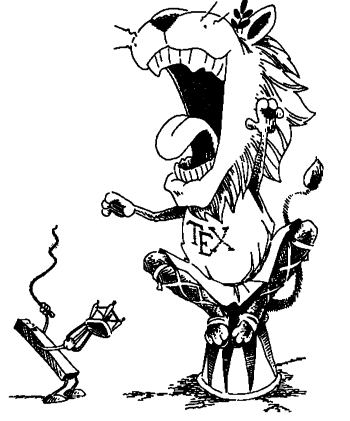
\includegraphics[width = \textwidth]{Chapter3.png}
		\caption{\TeX 的控制系列}\label{subfig:1b}
	\end{subfigure}
	\caption{子图模式测试1:2张图}\label{fig:subfig_test1}
\end{figure}

如\autoref{fig:subfig_test2}是有四张子图的模式,对子图进行交叉引用,如\autoref{subfig:2a}、\autoref{subfig:2b}、\autoref{subfig:2c}和\autoref{subfig:2d}。

\begin{figure}[htbp]
	\centering
	\begin{subfigure}[b]{.4\textwidth}
		\centering
		
\includegraphics[width = \textwidth]{Chapter4.png}
		\caption{字体}\label{subfig:2a}
	\end{subfigure}
	\begin{subfigure}[b]{.4\textwidth}
		\centering
		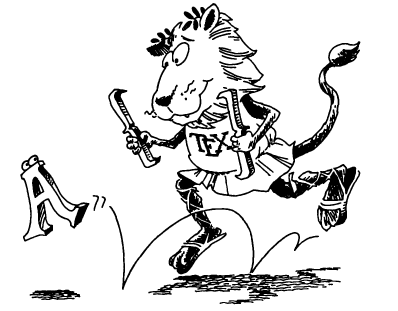
\includegraphics[width = \textwidth]{Chapter5.png}
		\caption{编组}\label{subfig:2b}
	\end{subfigure}
	\begin{subfigure}[b]{.4\textwidth}
		\centering
		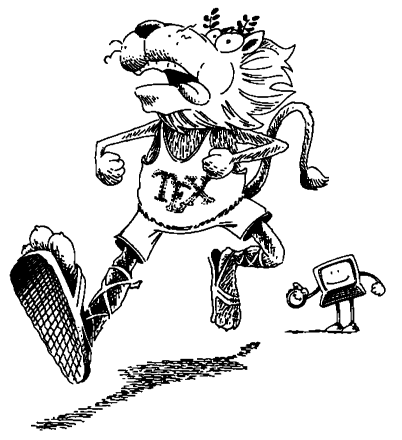
\includegraphics[width = \textwidth]{Chapter6.png}
		\caption{运行\TeX}\label{subfig:2c}
	\end{subfigure}
	\begin{subfigure}[b]{.4\textwidth}
		\centering
		
\includegraphics[width = \textwidth]{Chapter7.png}
		\caption{\TeX 工作原理}\label{subfig:2d}
	\end{subfigure}
	\caption{子图模式测试2:4张图}\label{fig:subfig_test2}
\end{figure}

\subsection{数学模式测试}
数学模式测试,主要测试数学字体,编号和交叉引用。这里首先推荐使用\texttt{align}和\texttt{align*}数学模式环境,大多数行间数学模式只需要用这个环境就可以了。

交叉引用测试,如交引用命令{\ttfamily \textbackslash eqref}和\texttt{\textbackslash ref}命令的区别。如公式\eqref{eq:test1},公式\ref{eq:test1}显示,\texttt{\textbackslash eqref}命令比\texttt{\textbackslash ref}命令的应用结果多了个括号。

如公式\eqref{eq:test3}是单行公式环境,查看公式\eqref{eq:test3}和\eqref{eq:test1}之间的区别,好像在单行公式中没什么区别。
\begin{align}\label{eq:test3}
	f(x) = 2(x + 1)^{2} - 1
\end{align}

\texttt{align}公式环境,用在单行中。
\begin{align}\label{eq:test1}
	f(x) = 2(x + 1)^{2} - 1
\end{align}

在这里,中间插入一些文字以形成段落,查看行间公式与上下文之间的间隙。
\begin{align*}
	f(x) = 2(x + 1)^{2} - 1
\end{align*}
在这里,中间插入一些文字以形成段落,查看行间公式与上下文之间的间隙。下一个公式\eqref{eq:test2}是一个公式组,它在“=”位置对齐。
\begin{align}\label{eq:test2}
	f(x) & = 2(x + 1)^{2} - 1\\
		 & = 2(x^{2} + 2x +1)-1\\
		 & = 2x^{2} + 4x + 1
\end{align}


\section{关于引用}
图表的引用通过{\ttfamily \textbackslash autoref} 命令即可,使用ST LaTeXTools 插件还能自动补全。如果要修改前缀,那么就用{\ttfamily \textbackslash recnewcommand \textbackslash figureautorefname\{好图\}}即可,详见hyperref宏包说明。

\section{出现的问题}
\subsection{\textbackslash texttt}
在这里发现一个问题,在下面的例子中可以发现,在中文中使用\textbackslash texttt\{\}命令时,前面的汉字与接下来的英文单词的空隙明显比接下来单词跟汉字的间隙要大,但是其它命令没有什么问题。

\begin{center}
\noindent 问题\texttt{问题}问题,问题\textbackslash\texttt{问题}问题。\\
问题\texttt{ref} 问题,问题\texttt{\textbackslash ref} 问题。\\
问题\textbf{ref}问题,问题\textbf{\textbackslash ref}问题。\\
问题\textsf{ref}问题,问题\textsf{\textbackslash ref}问题。\\
problem \texttt{ref} problem,problem \texttt{\textbackslash ref} problem.\\
problem \textbf{ref} problem,problem \textbf{\textbackslash ref} problem.\\
problem \textsf{ref} problem,problem \textsf{\textbackslash ref} problem.
\end{center}

原来的编译环境为texlive 2014,编译环境改为texlive 2015后,问题解决。


% !TEX root = ../main.tex

\chapter{三角贝赛尔曲面片表示的精确自由变形概述}
本文基于精确自由变形,并在此基础上进行了改进。所以我们先来看一下精确自由变形的大致思路。

\section{定义变形空间}
精确自由变形选用B样条体作为变形空间,记作$\mathbf R(u,v,w)$:
\begin{equation}
	\footnotesize
	{\mathbf R}(u,v,w) 
	= \sum_{i=0}^{m_u-1}\sum_{j=0}^{m_v-1}\sum_{k=0}^{m_w-1} {\mathbf
	R}_{ijk}N_{i,n_u}(u)N_{j,n_v}(v)N_{k,n_w}(w)
	\label{equ:Ruvw}
\end{equation}
其中,$n_u$、$n_v$、$n_w$与$m_u$、$m_v$、$m_w$分别表示B样条体三个维度上的阶数与控制顶点个数。$\{\mathbf R_{ijk}\}_{i=0,\hspace{6 pt} j=0,\hspace{8 pt} k=0}^{m_u-1,m_v-1,m_w-1}$表示$m_u\times m_v\times m_w$个控制顶点。$\{N_{i,n_u}(u)\}_{i=0}^{m_u-1}$, $\{N_{j,n_v}(v)\}_{j=0}^{m_v-1}$ 和 $\{N_{k,n_w}(w)\}_{k=0}^{m_w-1}$是B样条基函数。

此B样条体三个维度上的节点微量分别是$\{u_i\}^{n_u+m_u}_{i=0}$, $\{v_i\}^{n_v+m_v}_{j=0}$ 和 $\{w_k\}^{n_k+m_k}_{k=0}$。由此定义的三维区域$[u_i, u_{i+1}] \times [v_j, v_{j+1}] \times [w_k, w_{k+1}]$我们称之为节点盒。



\section{引言}
以下是一个测试用的列表环境,内容不要在意。\footnote{正文中中脚注命令测试,长脚注情况:这包括如下事实:“未经本人同意,监听、录制或转播私人性质的谈话或秘密谈话;未经本人同意,拍摄、录制或转播个人在私人场所的形象”}

这里测试列表标签功能的交叉引用格式\ref{itm:11},\ref{itm:12},\ref{itm:13},\ref{itm:14},分别表示第一至第四层级的itemize系列的交叉引用情况。
\begin{enumerate}
	\item 第一级列表\label{itm:11}
	\begin{enumerate}
		\item 第二级列表\label{itm:12}
	\end{enumerate}
\end{enumerate}

\begin{itemize}
	\item 第一级列表
	\begin{itemize}
		\item 第二级列表
	\end{itemize}
\end{itemize}

\section{浮动体测试}
\subsection{插图测试}
如\autoref{fig:first_image_tset}是对此模版的第一张插图测试。

\begin{figure}[htbp]
	\centering
	
\includegraphics[width = 0.5\linewidth]{Chapter1.png}
	\caption{第一张插图测试}\label{fig:first_image_tset}
\end{figure}

\subsection{表格测试}

\subsubsection{array宏包tabular表格环境测试}
如\autoref{tab:first_table_test}是对array宏包的tabular表格环境测试。
\begin{table}[htbp]
	\centering
	\caption{这是一个用tabular环境的测试用的表格}\label{tab:first_table_test}
    \begin{tabular}{lrr}
    \toprule
    \textbf{行星}     & \textbf{赤道半径}km & \textbf{公转周期}d \\
    \midrule
    水星     & 2.439  & 87.9 \\
    金星     & 6.1    & 224.682 \\
    地球     & 6378.14 & 365.24 \\
    \bottomrule
    \end{tabular}%
\end{table}

\subsubsection{tabu宏包表格环境测试}
如\autoref{tab:tabu_test_1}是对tabu宏包的tabu表格环境测试。在这里表格命令与\autoref{tab:first_table_test}的命令相同,只是tabular环境改成了tabu环境。
\begin{table}[htbp]
	\centering
	\caption{这是一个用tabu环境的测试用的表格}\label{tab:tabu_test_1}
    \begin{tabu}{lrr}
    \toprule
    \textbf{行星}     & \textbf{赤道半径}km & \textbf{公转周期}d \\
    \midrule
    水星     & 2.439  & 87.9 \\
    金星     & 6.1    & 224.682 \\
    地球     & 6378.14 & 365.24 \\
    \bottomrule
    \end{tabu}%
\end{table}

\autoref{tab:tabu_test_2}对tabu to表格的x列模式进行测试。在表格导言区中设置为X[1]X[2]X[2],表示这三列表格的列宽比值为1:2:2,总的表格宽度由tabu to环境设置,这里设置为0.6\textbackslash linewidth。相比于tabular环境,tabu环境的列宽设置方便许多。
\begin{table}[htbp]
	\centering
	\caption{tabu环境测试表格---X列模式}\label{tab:tabu_test_2}
    \begin{tabu} to 0.6\linewidth{X[1]X[2]X[2]}
    \toprule
    \textbf{行星}     & \textbf{赤道半径}km & \textbf{公转周期}d \\
    \midrule
    水星     & 2.439  & 87.9 \\
    金星     & 6.1    & 224.682 \\
    地球     & 6378.14 & 365.24 \\
    \bottomrule
    \end{tabu}%
\end{table}

特别需要注意的是,longtabu是基于longtable宏包开发的,所以在zjuthesis.cls文件中已经插入了longtable宏包。longtable环境的所有功能都可以在longtabu中使用,如\textbackslash endhead,\textbackslash endfirsthead,\textbackslash endfoot,\textbackslash endlastfoot,和\textbackslash caption等。具体用法请参见longtable和tabu宏包的相应文档。
\begin{longtabu}{lccc}
\caption{材料弹性模量及泊松比}\label{tab:tabu_test_3}\\
\toprule
名  称   & 弹性模量E/Gpa & 切变模量G/Gpa & 泊松比$\mu$ \\
\midrule%
\endfirsthead
\caption{材料弹性模量及泊松比(续)}\\
\toprule
名  称   & 弹性模量E/Gpa & 切变模量G/Gpa & 泊松比$\mu$ \\
\midrule%
\endhead
\bottomrule%
\endfoot
镍铬钢、合金钢 & 206    & 79.38  & 0.3 \\
碳 钢    &  196~206 & 79     & 0.3 \\
\end{longtabu}%

\subsection{子图}

如\autoref{fig:subfig_test1}是有两张子图的模式,对子图进行交叉引用,如\autoref{subfig:1a}和\autoref{subfig:1b}。

\begin{figure}[htbp]
	\centering
	\begin{subfigure}[b]{.4\textwidth}
		\centering
		
\includegraphics[width = \textwidth]{Chapter2.png}
		\caption{书籍排版与普通排版}\label{subfig:1a}
	\end{subfigure}
	\quad
	\begin{subfigure}[b]{.4\textwidth}
		\centering
		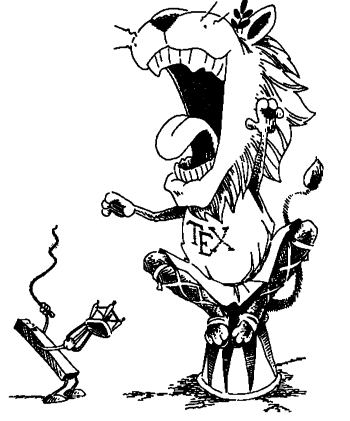
\includegraphics[width = \textwidth]{Chapter3.png}
		\caption{\TeX 的控制系列}\label{subfig:1b}
	\end{subfigure}
	\caption{子图模式测试1:2张图}\label{fig:subfig_test1}
\end{figure}

\begin{figure}[htbp]
	\centering
	\begin{subfigure}[b]{.4\textwidth}
		\centering
		
\includegraphics[width = \textwidth]{Chapter4.png}
		\caption{字体}\label{subfig:2a}
	\end{subfigure}
	\begin{subfigure}[b]{.4\textwidth}
		\centering
		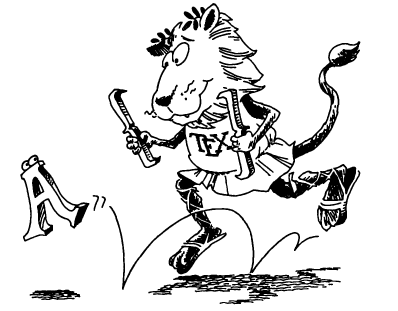
\includegraphics[width = \textwidth]{Chapter5.png}
		\caption{编组}\label{subfig:2b}
	\end{subfigure}
	\begin{subfigure}[b]{.4\textwidth}
		\centering
		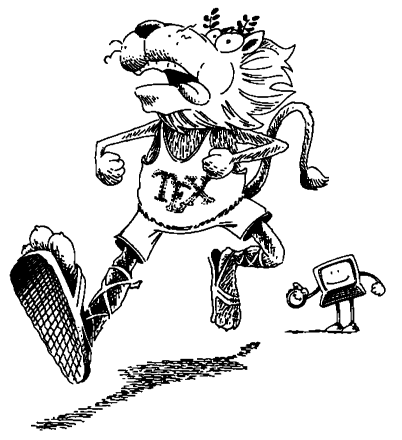
\includegraphics[width = \textwidth]{Chapter6.png}
		\caption{运行\TeX}\label{subfig:2c}
	\end{subfigure}
	\begin{subfigure}[b]{.4\textwidth}
		\centering
		
\includegraphics[width = \textwidth]{Chapter7.png}
		\caption{\TeX 工作原理}\label{subfig:2d}
	\end{subfigure}
	\caption{子图模式测试2:4张图}\label{fig:subfig_test2}
\end{figure}

\subsection{数学模式测试}
数学模式测试,主要测试数学字体,编号和交叉引用。这里首先推荐使用\texttt{align}和\texttt{align*}数学模式环境,大多数行间数学模式只需要用这个环境就可以了。

交叉引用测试,如交引用命令{\ttfamily \textbackslash eqref}和\texttt{\textbackslash ref}命令的区别。如公式\eqref{eq:test1},公式\ref{eq:test1}显示,\texttt{\textbackslash eqref}命令比\texttt{\textbackslash ref}命令的应用结果多了个括号。

如公式\eqref{eq:test3}是单行公式环境,查看公式\eqref{eq:test3}和\eqref{eq:test1}之间的区别,好像在单行公式中没什么区别。
\begin{align}\label{eq:test3}
	f(x) = 2(x + 1)^{2} - 1
\end{align}

\texttt{align}公式环境,用在单行中。
\begin{align}\label{eq:test1}
	f(x) = 2(x + 1)^{2} - 1
\end{align}

\begin{align*}
	f(x) = 2(x + 1)^{2} - 1
\end{align*}
在这里,中间插入一些文字以形成段落,查看行间公式与上下文之间的间隙。下一个公式\eqref{eq:test2}是一个公式组,它在“=”位置对齐。
\begin{align}\label{eq:test2}
	f(x) & = 2(x + 1)^{2} - 1\\
		 & = 2(x^{2} + 2x +1)-1\\
		 & = 2x^{2} + 4x + 1
\end{align}


\section{关于引用}
图表的引用通过{\ttfamily \textbackslash autoref} 命令即可,使用ST LaTeXTools 插件还能自动补全。如果要修改前缀,那么就用{\ttfamily \textbackslash recnewcommand \textbackslash figureautorefname\{好图\}}即可,详见hyperref宏包说明。

% !TEX root = ../main.tex

\chapter{三角均匀剖分算法}
如上文所述,光滑自由变形需将模型沿节点盒切割,并将得到的非三角形的面片三角化。这一过程很可能产生狭长三角形或者蜕化三角形,如\autoref{subfig:clip_compare0}所示,颜色越红表示三角形质量越差。过多的此类三角形不仅会浪费计算资源,还可能带来其它数值计算方面的问题。

另一方面,如第\autoref{sec:clip_against_knot_box}节所述,“沿节点盒切割”这一步骤在光滑自由变形中的作用并非保证变形结果精确,而是将原始三角面片切割成较小的三角形,从而减少变形结果的拟合误差。若略去这一步骤,算法仍能继续,只不过结果拟合误差会增加。也就是说,在光滑自由变形中,沿节点盒切割的目的是减少拟合误差,进一步分析,“沿节点盒切割”这一步骤有两个要素:“沿节点盒”和“切割”,并且导致拟合误差减少的要素是“切割”,而不是“沿节点盒”。因此,换一种切割方法,并不一定要沿节点盒,只要将较大的三角形切割成多个较小的子三角形,仍能起到与“沿节点盒切割”相同的效果。

而且,我们通过更进一步的观察发现,在光滑自由变形中,跨节点盒的三角面片只要足够小,其变形后在精度上的误差,相对于在节点盒内的三角面片而言,并不会显著增加。

因此,本文尝试提出一种更好的三角形分割算法,以替换光滑自由变形中的“沿节点盒切割”这一步骤。新算法不再沿节点盒切割三角面片,而是将三角面片在满足以下两个要求的情况下分割成多个子三角形:
\begin{enumerate}
    \item 所有子三角形的三边长都尽可能相等。以得到形状尽可能接近正三角形,且面积尽可能相同的子三角形。
    \item 所有子三角形的顶点均不可位于其它子三角形的边上。以避免变形后产生裂缝。
\end{enumerate}

我们的新算法相比原来的沿节点盒分割的算法而言有两点优势:
\begin{enumerate}
        \item 切分出来的子三角形尽可能“正”,不会产生新的狭长或蜕化的三角形。
        \item 参数$l$使得用户可以控制产生的子三角形的大小,进而根据自己的需求和硬件的性能通过改变$l$大小选择合适的变形精度。
\end{enumerate}

\section{算法实现} \label{clip_algorithm}
首先我们先定义一些符号以方便描述算法实现。$l$,$t$为算法的输入,$l$表示子三角形边长的期望值,算法分割产生的子三角形的三边的长度需尽可能接近$l$。$t$表示待分割的三角面片。$\{e_i\}^{2}_{i=0}$为$t$的三条边。$\{len_i\}^{2}_{i=0}$代表三边的边长。$t$的每条边会被均匀分成$\lceil len_i/l \rceil$段。$p_{ij}$表示三角形第i条边的第j个分割点。

算法流程:
\begin{enumerate}
    \item 找出三角面片最小的内角$\alpha$,\autoref{subfig:clip1}中用红色边标识出了角$\alpha$。不妨假定角$\alpha$的两条边为$e_0$, $e_1$。

    \item 将$e_0$、$e_1$分别均匀分成$\lceil len_0/l \rceil$、$\lceil len_1/l \rceil$段,分别产生的切割点的有序集合\footnote{一条边上的切割点的有序集合包括边上首尾端点}为$\{p_{0j}\}^{\lceil len_0/l \rceil}_{j=0}$、$\{p_{1j}\}^{\lceil len_1/l \rceil}_{j=0}$,且$j$沿角$\alpha$的顶点至另一端点方向依次增长。分割点如\autoref{subfig:clip2}所示。

    \item 将子三角形$p_{00}p_{01}p_{11}$分割下来,剩余部分如\autoref{subfig:clip3}红色部分所示。

    \item 剩下的部分是一个类似于梯形的四边形,如\autoref{subfig:clip3}中红色部分所示。如果$\lceil len_0/l \rceil == \lceil len_1/l \rceil$,我们依次将四边形$\{p_{0j}p_{1j}p_{1(j+1)}p_{0(j+1)}\}^{\lceil len_0/l \rceil - 1}_{j=0}$分割成子三角形\footnote{将一个上下底边较长的类梯形的四边形分割为三角形的过程较为简单,在此略过不表},如\autoref{subfig:clip6}、\autoref{subfig:clip9}所示,直到所有四边形分割完毕,然后直接跳转到步骤\ref{CVT};否则\footnote{既$\lceil len_0/l \rceil \ne \lceil len_1/l \rceil$},我们依次将四边形$\{p_{0j}p_{1j}p_{1(j+1)}p_{0(j+1)}\}^{min(\lceil len_0/l \rceil, \lceil len_1/l \rceil) - 2}_{j=0}$分割成子三角形,剩余部分如\autoref{subfig:clip16}所示。\label{recursion}

    \item \autoref{subfig:clip16}中剩余部分若逆时针旋转90度,我们可以发现剩余部分和\autoref{subfig:clip3}类似。所以我们递归的进行步骤\ref{recursion},直到三角形分割完毕。\label{recursion2}

    \item 对分割结果进行5次CVT优化\cite{du1999},使子三角形边长更加接近$l$。\label{CVT}
\end{enumerate}

在步骤\ref{recursion2}中,递归到最后阶段,可能会出现步骤\ref{recursion}处理不了的特殊情况。但是特殊情况的类型不会很多,所以我们枚举出了每一种特殊情况所对应的分割方案。

\begin{figure}[htbp]
	\centering
	\begin{subfigure}[b]{.32\textwidth}
		\centering
		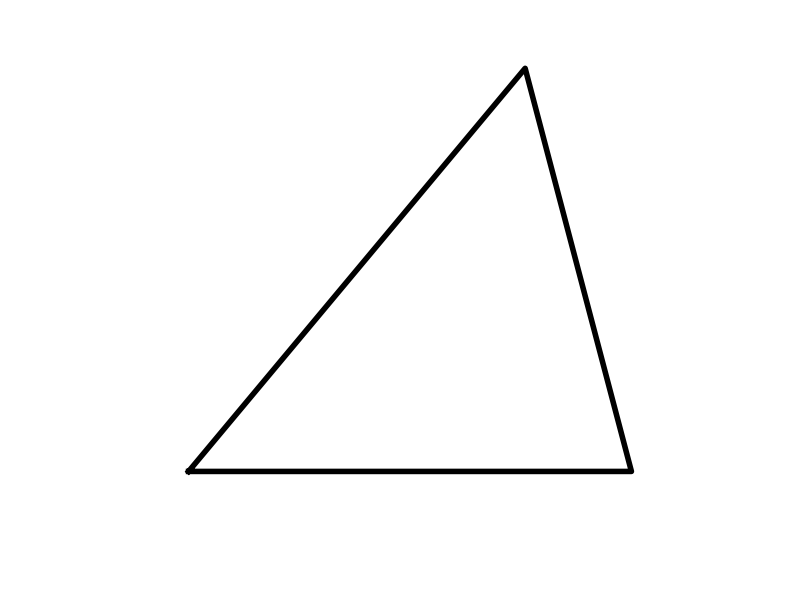
\includegraphics[width = \textwidth]{clip_figure0.png}
		\caption{初始三角面片}\label{subfig:clip0}
	\end{subfigure}
	\begin{subfigure}[b]{.32\textwidth}
		\centering
		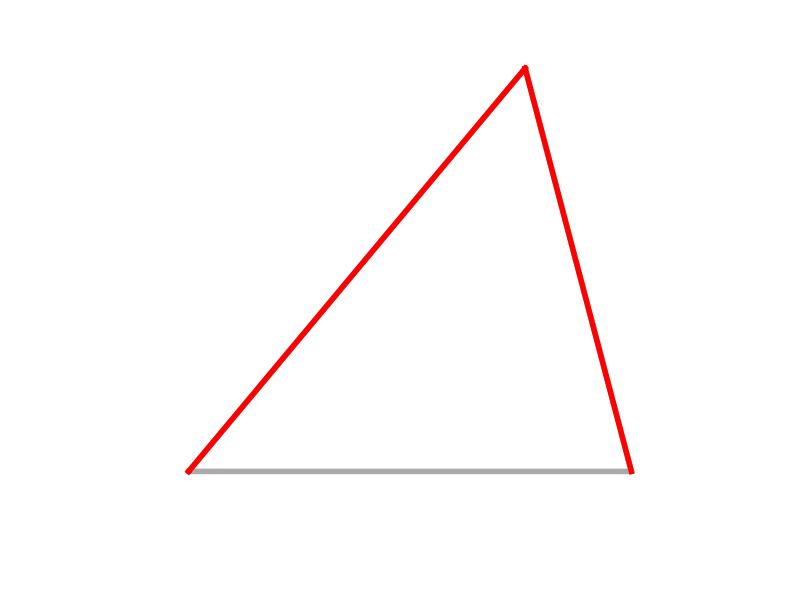
\includegraphics[width = \textwidth]{clip_figure1.png}
		\caption{初始三角面片}\label{subfig:clip1}
	\end{subfigure}
	\begin{subfigure}[b]{.32\textwidth}
		\centering
		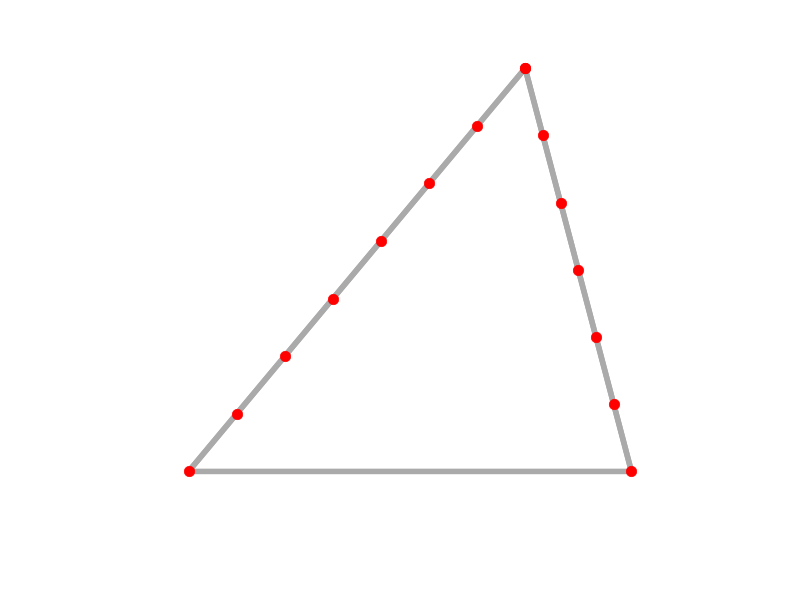
\includegraphics[width = \textwidth]{clip_figure2.png}
		\caption{分割最小角$\alpha$的两条边}\label{subfig:clip2}
	\end{subfigure}

	\begin{subfigure}[b]{.32\textwidth}
		\centering
		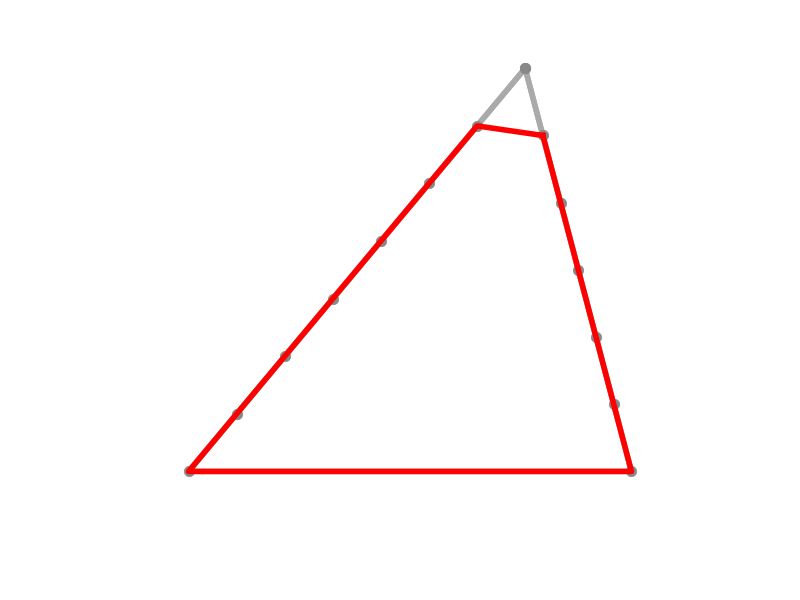
\includegraphics[width = \textwidth]{clip_figure3.png}
		\caption{切割第一个子三角形}\label{subfig:clip3}
	\end{subfigure}
	\begin{subfigure}[b]{.32\textwidth}
		\centering
		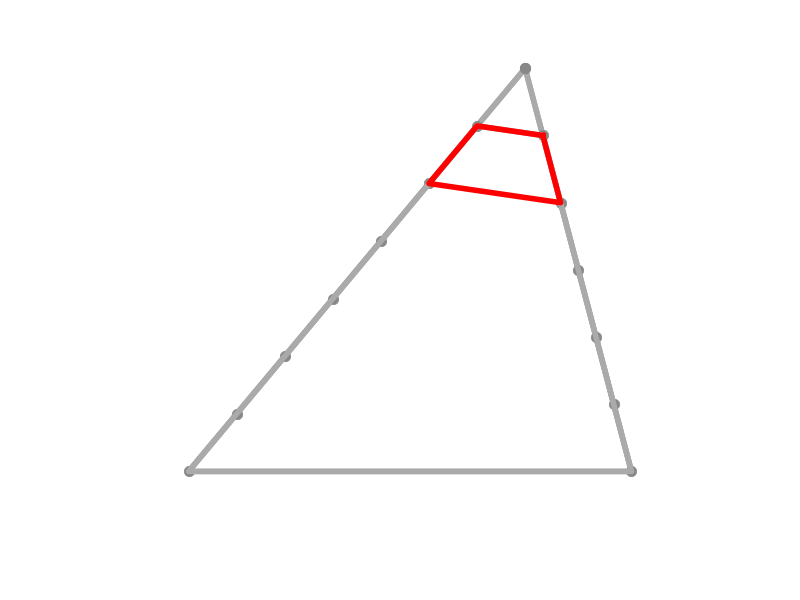
\includegraphics[width = \textwidth]{clip_figure4.png}
		\caption{第一个待分割层}\label{subfig:clip4}
	\end{subfigure}
	\begin{subfigure}[b]{.32\textwidth}
		\centering
		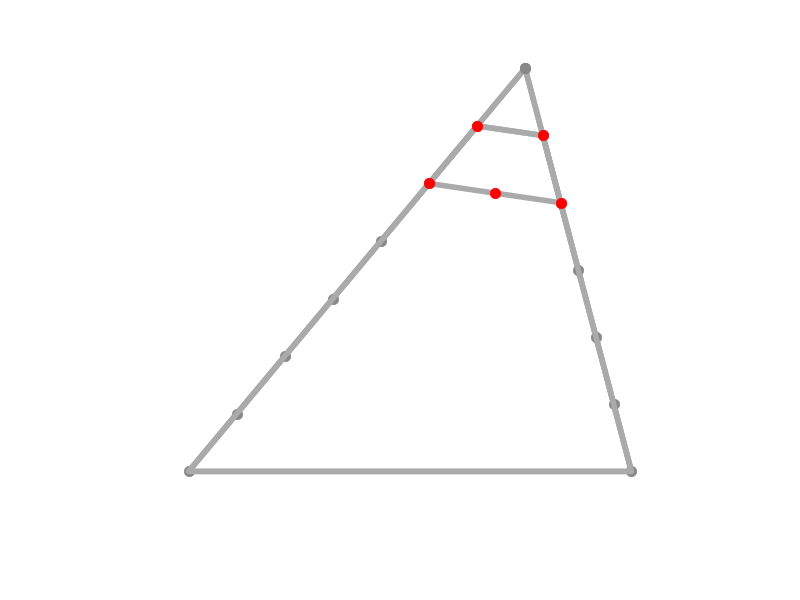
\includegraphics[width = \textwidth]{clip_figure5.png}
		\caption{分割待分割层的上下底边}\label{subfig:clip5}
	\end{subfigure}

	\begin{subfigure}[b]{.32\textwidth}
		\centering
		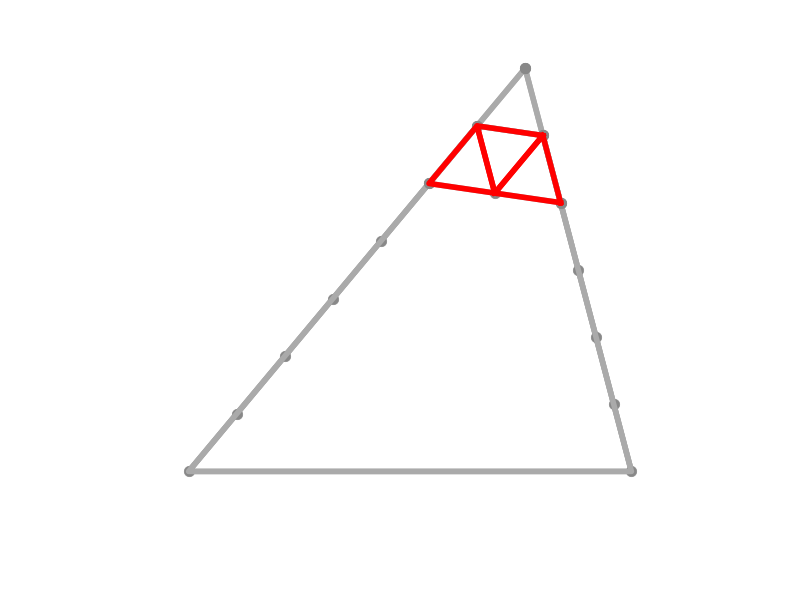
\includegraphics[width = \textwidth]{clip_figure6.png}
		\caption{分割待分割层的上下底边}\label{subfig:clip6}
	\end{subfigure}
	\begin{subfigure}[b]{.32\textwidth}
		\centering
		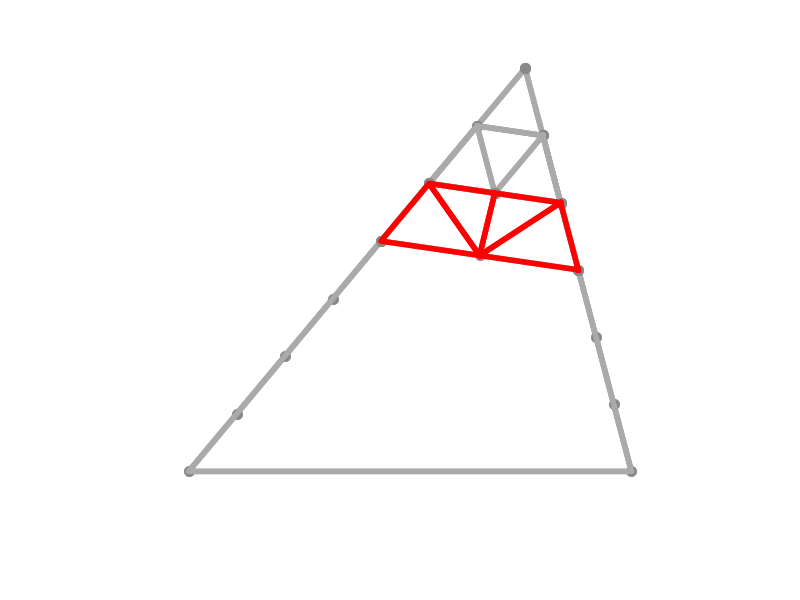
\includegraphics[width = \textwidth]{clip_figure9.png}
		\caption{分割待分割层的上下底边}\label{subfig:clip9}
	\end{subfigure}
	\begin{subfigure}[b]{.32\textwidth}
		\centering
		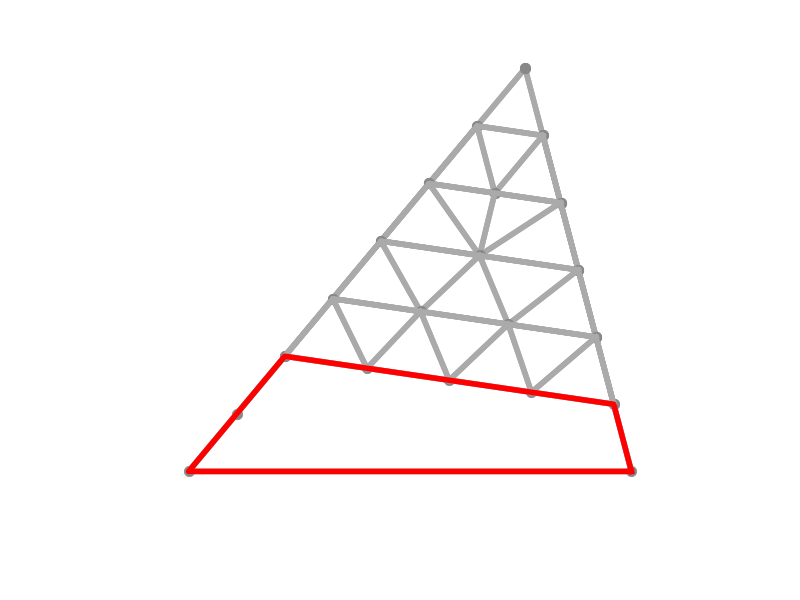
\includegraphics[width = \textwidth]{clip_figure16.png}
		\caption{继续分割红色部分}\label{subfig:clip16}
	\end{subfigure}

	\begin{subfigure}[b]{.32\textwidth}
		\centering
		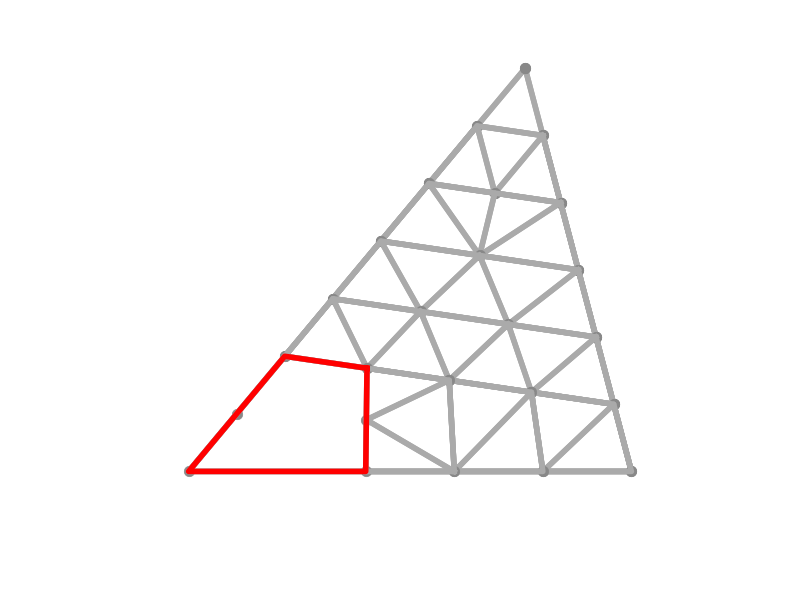
\includegraphics[width = \textwidth]{clip_figure26.png}
		\caption{对特殊情况进行处理}\label{subfig:clip26}
	\end{subfigure}
	\begin{subfigure}[b]{.32\textwidth}
		\centering
		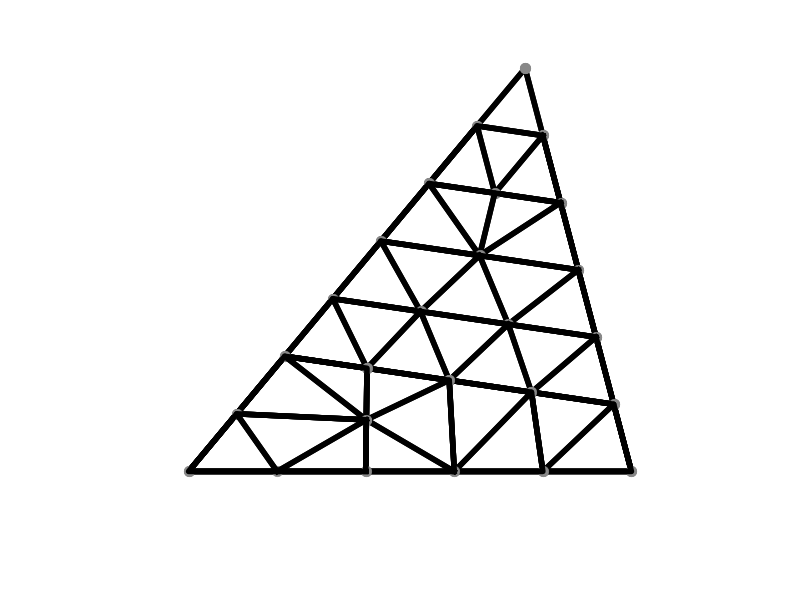
\includegraphics[width = \textwidth]{clip_figure33.png}
		\caption{分割结果}\label{subfig:clip33}
	\end{subfigure}
	\begin{subfigure}[b]{.32\textwidth}
		\centering
		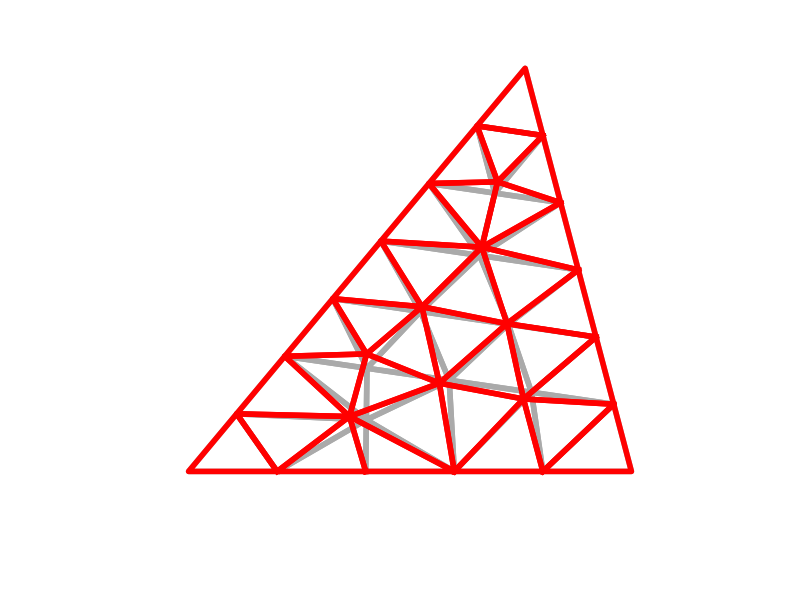
\includegraphics[width = \textwidth]{clip_figure34.png}
		\caption{对结果进行CVT优化}\label{subfig:clip34}
	\end{subfigure}
	\caption{均匀三角剖分算法}\label{fig:clip}
\end{figure}

CVT优化\cite{du1999}可以使分割更加均匀。且该过程可以迭代进行,使分割结果越来越均匀。\autoref{fig:CVT}展示了迭代过程,红色是优化之后的结果,灰色的是优化之前的。我们可以发现,从第5次迭代开始,每次迭代后的收益很小。所以我们最终选择对原始分割结果进行5次CVT迭代优化。

\begin{figure}[htbp]
	\centering
	\begin{subfigure}[b]{.49\textwidth}
		\centering
		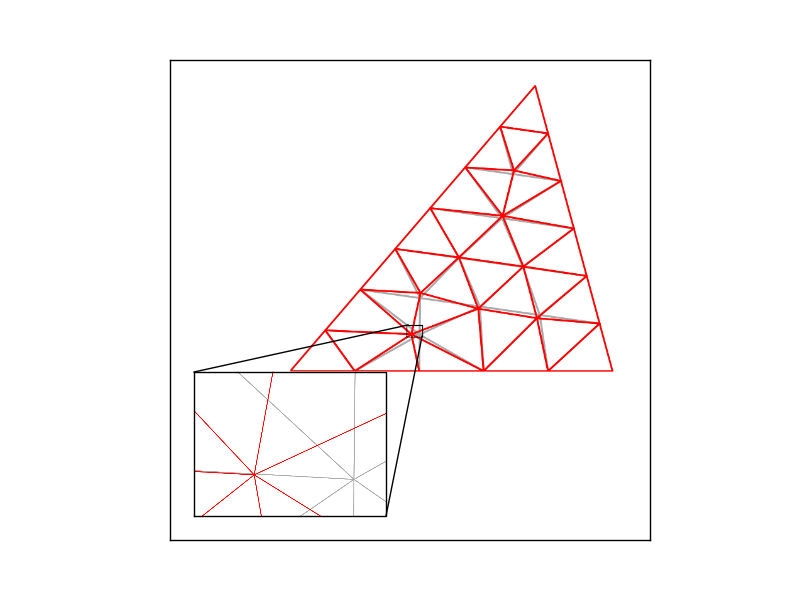
\includegraphics[width = \textwidth]{cvt_for_paper0.png}
		\caption{第1次CVT优化}
	\end{subfigure}
	\begin{subfigure}[b]{.49\textwidth}
		\centering
		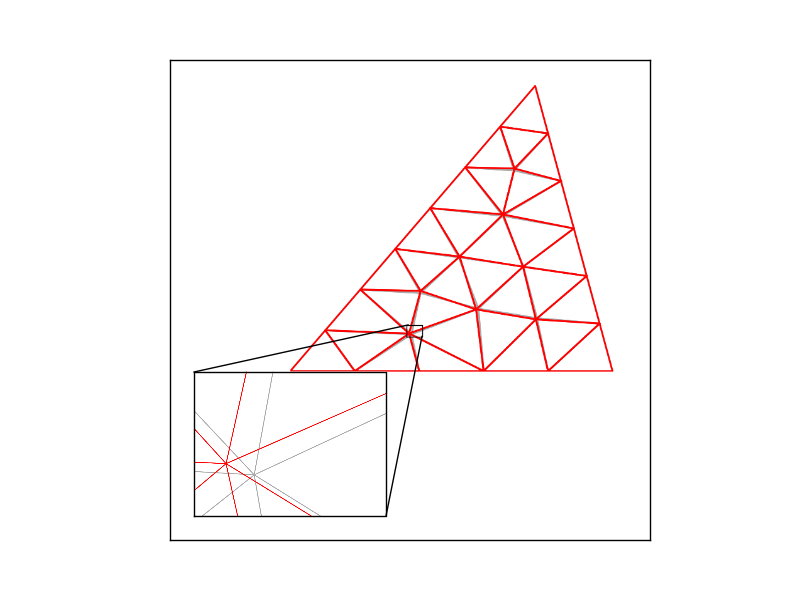
\includegraphics[width = \textwidth]{cvt_for_paper1.png}
		\caption{第2次CVT优化}
	\end{subfigure}

	\begin{subfigure}[b]{.49\textwidth}
		\centering
		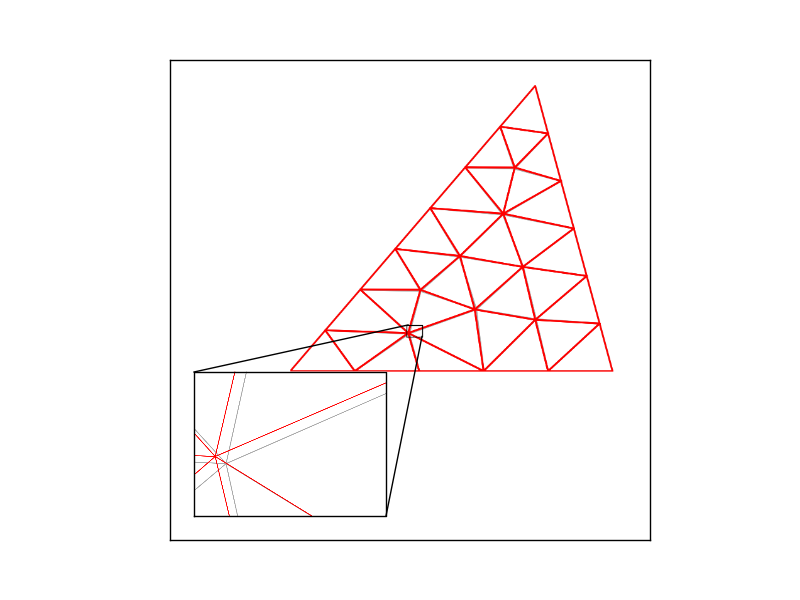
\includegraphics[width = \textwidth]{cvt_for_paper2.png}
		\caption{第3次CVT优化}
	\end{subfigure}
	\begin{subfigure}[b]{.49\textwidth}
		\centering
		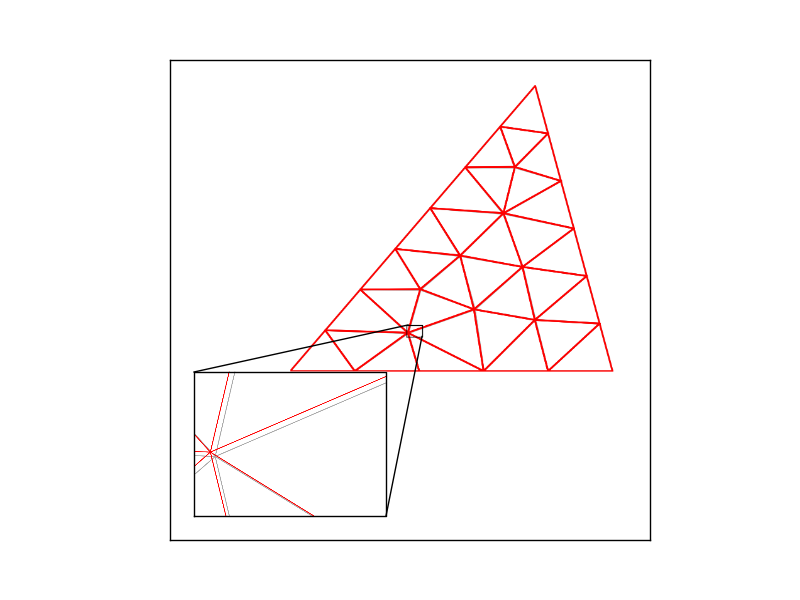
\includegraphics[width = \textwidth]{cvt_for_paper3.png}
		\caption{第4次CVT优化}
	\end{subfigure}

	\begin{subfigure}[b]{.49\textwidth}
		\centering
		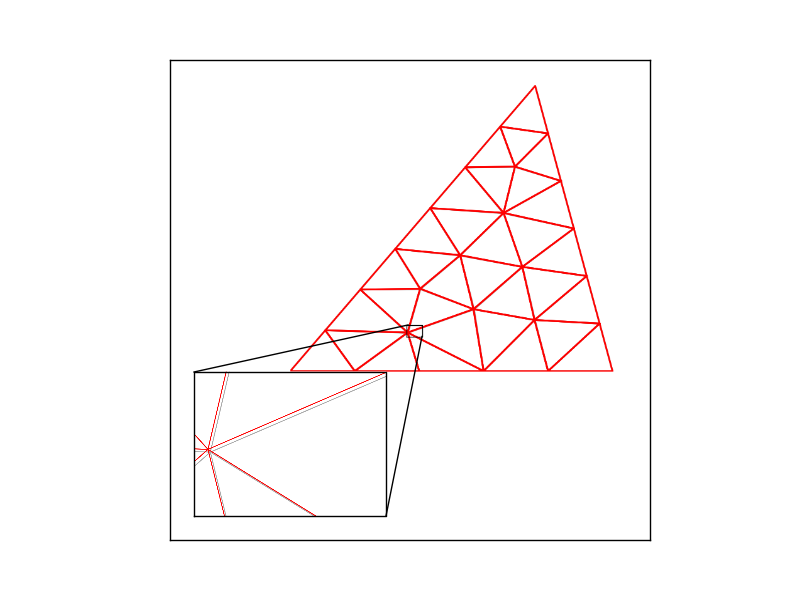
\includegraphics[width = \textwidth]{cvt_for_paper4.png}
		\caption{第5次CVT优化}
	\end{subfigure}
	\begin{subfigure}[b]{.49\textwidth}
		\centering
		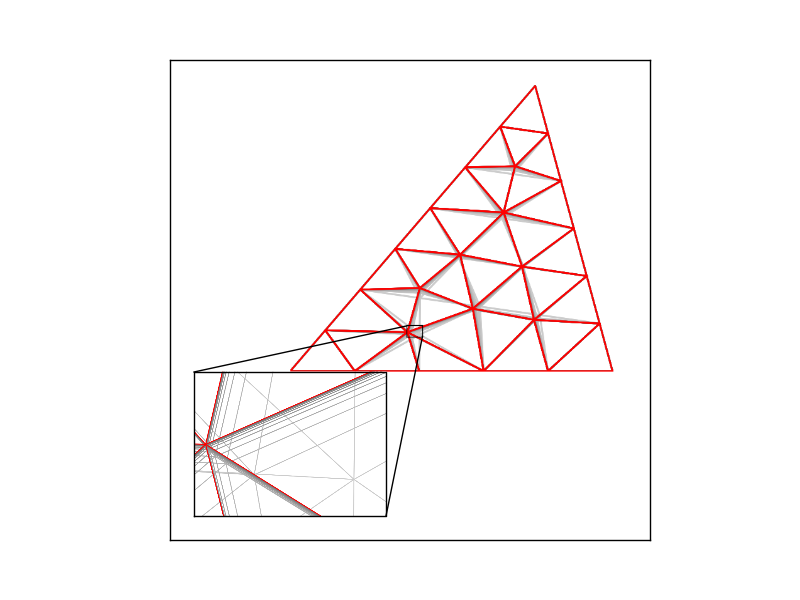
\includegraphics[width = \textwidth]{cvt_for_paper5.png}
		\caption{1~10次CVT优化}
	\end{subfigure}
    \caption{CVT优化结果} \label{fig:CVT}
\end{figure}

\section{关于$l$的讨论}
前文提到的$l$是一个很关键的参数,$l$不仅会影响算法效率、子三角形的质量\footnote{这里的质量表示接近正三角形的程度}、还能影响拟合得到的变形结果相对精确结果的拟合误差。但是,$l$并不是影响这些的根本因素,对分割后得到的子三角形的质量和算法效率产生直接影响的是子三角形的数目,而对变形结果的精度产生直接影响的是子三角形的平均面积\footnote{这两者在一定程度上是等价的,因为对于同一个三角形,剖分后得到的子三角形的数目趍,每个子三角形的面积就越小。}。$l$则通过改变子三角形数目或平均面积,间接地对算法效率、子三角形的质量、变形结果的精度产生影响。

定性的来说$l$越小,子三角形数目越多,面积越小,同时子三角形的质量越高,变形结果的误差越小,但算法的计算代价越高。为了进一步明确$l$对算法的影响,我们进行了一系列实验以定量的分析$l$。

实验选用了立方体模型,有12个面片,且模型被归一化到$[-1, 1]^3$。之所以选择由大三角面片组成的模型,是为了让三角面片随$l$变化切割出不同大小的子三角形。\autoref{fig:l-number}显示了$l$与子三角形数量的关系,蓝色表示以立方体为模型进行切割,立方体原始的三角面片平均面积为2.0;绿色表示以兔子玩偶为模型进行切割,兔子玩偶原始的三角面片平均面积为0.0007。从中我们可以发现由于兔子玩偶模型原始三角片面过小,当$l$大于某个值的时候,其不再被切割,子三角形的数目也保持不变,这样不利于我们探索$l$在变化过程中对变形算法产生的影响。而立方体由于原始三角面片较大,能随$l$变化切割出不同数目的子三角形。可以帮助我们更好的研究$l$对算法的影响。

变形空间的次数是$3\times3\times3$,控制顶点个数是$5\times5\times5$,变形空间范围是$[-1, 1]^3$。实验的自变量是$l$,由$0.1$增长到$2\sqrt{3}$\footnote{$2\sqrt{3}$为变形空间对角线长度}。因变量是算法效率、子三角形的质量和变形结果的精度。以下是实验结果。

%兔子模型的平均三角形面积为总表面积/三角形数目
%5.880918 / 8400 = 0.0007001092857142858
\begin{figure}[htbp]
	\centering
	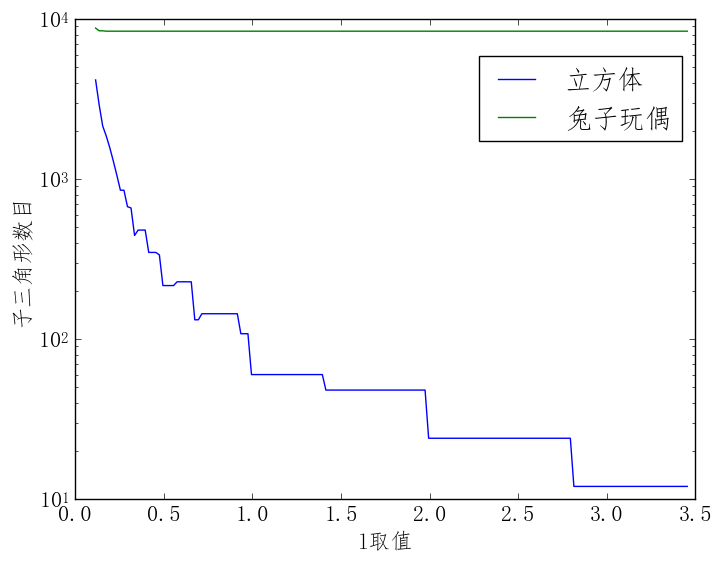
\includegraphics[width = 0.8\textwidth]{l-number.png}
	\caption{$l$取值-子三角形数目关系图}\label{fig:l-number}
\end{figure}

\subsection{算法效率}
从\autoref{fig:l-number}可以看出不同的$l$可能产生相同的分割结果,所以\autoref{fig:l-time0}中,$l$与算法运算时间的关系不是很直观。如前文所述,$l$通过影响子三角形数目,从而影响算法运算时间,所以我们直接探究子三角形数目和算法运算时间的关系。如\autoref{fig:l-time1}中所示,大体上来看,算法运行时间与子三角形数目呈线性正相关。

\begin{figure}[htbp]
	\centering
	\begin{subfigure}[b]{.45\textwidth}
	    \centering
	    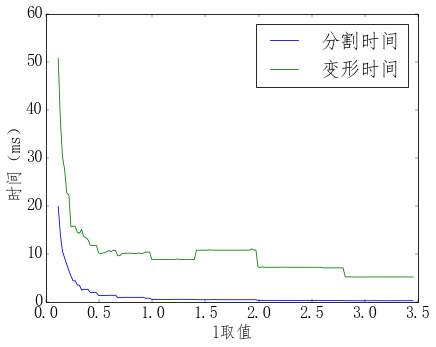
\includegraphics[width =\textwidth]{l-time0.png}
	    \caption{$l$取值-算法运行时间关系图}\label{fig:l-time0}
	\end{subfigure}
	\begin{subfigure}[b]{.45\textwidth}
	    \centering
	    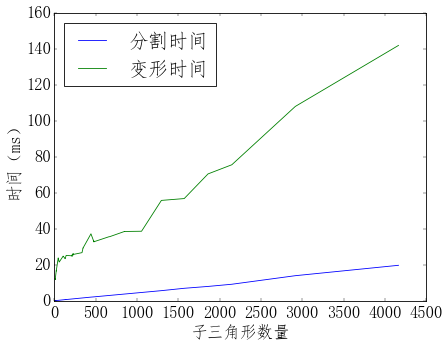
\includegraphics[width =\textwidth]{l-time1.png}
	    \caption{三角形数目-算法运行时间关系图}\label{fig:l-time1}
	\end{subfigure}
	\caption{$l$取值-算法效率}\label{fig:l-time}
\end{figure}

这部分数据说明当本文算法运行比较"卡"时,增加$l$值可以有效地加快算法响应速度。同时,可以指导用户根据硬件条件与编辑过程中对实时交互的依赖程度选择合适的$l$,如用户可以在编辑过程中选择较大的$l$,而在完成编辑,导出变形结果时选择较小的$l$,以兼顾精度和效率。

\subsection{子三角形质量}
    本节探讨$l$与子三角形质量之间的关系,在此之前,我们先明确本文中对于三角形质量的定义:三角形质量表示一个三角形从形状上接近正三角形的程度,三角形越接近正三角形,其质量越差,反之亦然。

    以上定义是对三角形质量定性的描述,我们需要进一步确定一个指标来衡量三角形的质量。有很多指标都可以衡量三角形质量\cite{pebay2003},我们选取了其中计算量较少的一个$q(t)=r_t/max(\{e_i\}^{2}_{i=0})$,即三角形外接圆的半径除以其最长边长度。该指标的取值范围是$(0, \frac{\sqrt{3}}{2}]$,当三角形$t$为正三角形时,$q(t)$取到最大值$\frac{\sqrt{3}}{2}$;三角形$t$越狭长,$q(t)$的值越接近0。为了更直观的用该指标表示三角形质量,我们修改将$q(t)$修改为$q(t)=r_t/max(\{e_i\}^{2}_{i=0})*2\sqrt{3}$,使其取值范围归一化到$(0, 1]$。\autoref{fig:triangle_quality_compare}可视化了两种三角形分割方法产生的三角形的质量,可以很明显的观察到沿节点盒切割方法生产的大量狭长三角形,而本文方法切割产生的三角形及其匀称。可见在这方面,本文方法明显占优。

\begin{figure}[htbp]
	\centering
	\begin{subfigure}[b]{.3\textwidth}
		\centering
		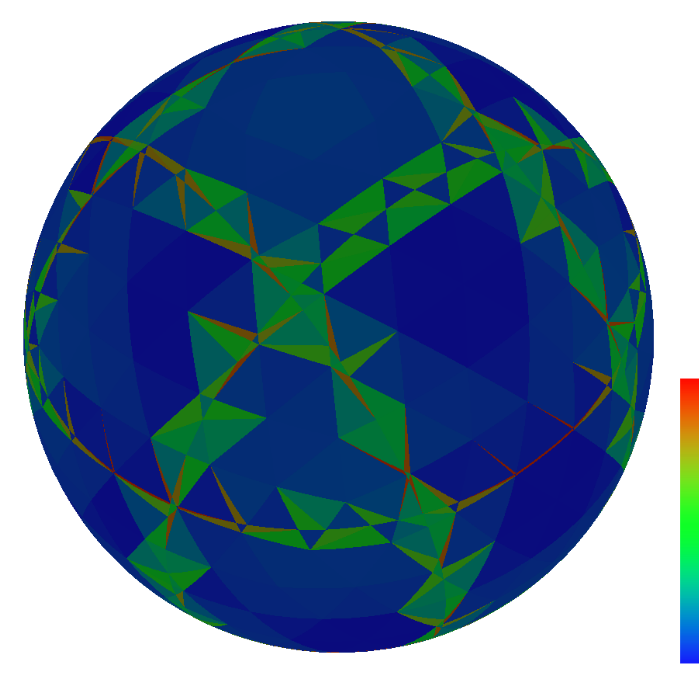
\includegraphics[width = \textwidth]{clip_compare0.png}
		\caption{沿节点盒切割}\label{subfig:clip_compare0}
	\end{subfigure}%
	\begin{subfigure}[b]{.3\textwidth}
		\centering
		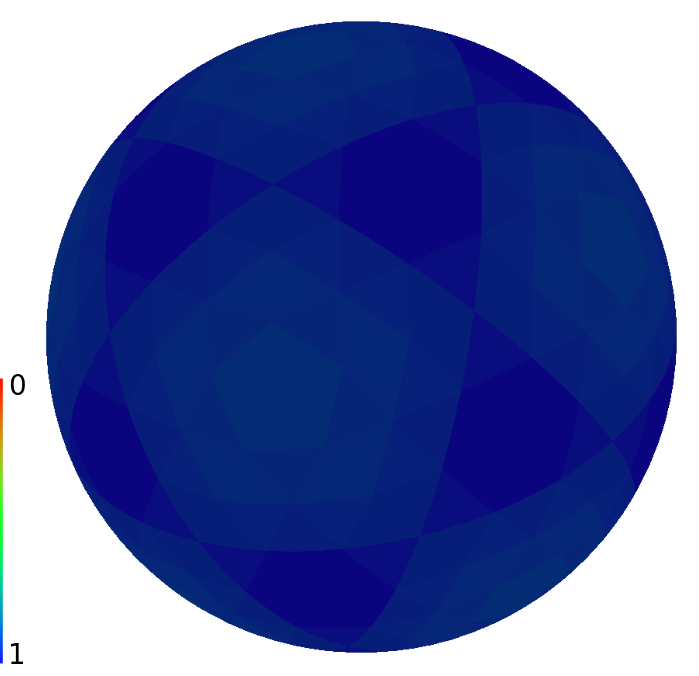
\includegraphics[width = \textwidth]{clip_compare1.png}
		\caption{本文方法}\label{subfig:clip_compare1}
	\end{subfigure}
	\caption{两种切割算法产生的子三角形的质量对比}\label{fig:triangle_quality_compare}
\end{figure}

不同的$l$对三角形质量的影响如\autoref{fig:l-quality}所示。我们分别作了$l$取值、子三角形数目与子三角形质量的关系图。可见$l$越小,三角形质量越高。但是由于切割算法中存在取整操作,所以\autoref{fig:l-quality}存在许多跳变的地方。同时我们可以从\autoref{subfig:l-quality1}中发现,当三角形数目达到某一临界值时,三角形质量不再显著增加。在该例子中这个值672,既每个原始三角形都被分成了56个小三角形。我们通过进一步实验发现,原始三角形的质量越差,该临界值就越大。

\begin{figure}[htbp]
	\centering
	\begin{subfigure}[b]{.45\textwidth}
		\centering
		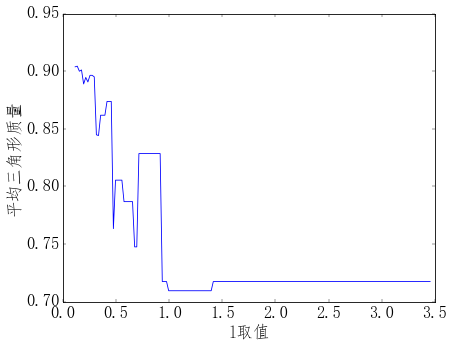
\includegraphics[width = \textwidth]{l-quality0.png}
		\caption{$l$取值-子三角形质量关系图}\label{subfig:l-quality0}
	\end{subfigure}%
	\begin{subfigure}[b]{.45\textwidth}
		\centering
		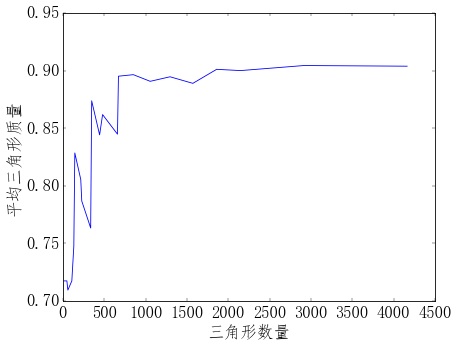
\includegraphics[width = \textwidth]{l-quality1.png}
		\caption{子三角形数目-子三角形质量关系图}\label{subfig:l-quality1}
	\end{subfigure}
	\caption{$l$取值-子三角形的质量对比}\label{fig:l-quality}
\end{figure}

\subsection{变形结果精度}
相比于光滑自由变形,本文方法会产生跨节点盒的子三角形。这些三角形会引入额外的误差。但是只要子三角足够小,误差就能控制在可接受范围内。我们同样做了实验以验证$l$取值与变形误差的关系。从\autoref{fig:l-error}中可以看出,变形结果的几何误差基本与子三角形面积呈线性正相关。
\begin{figure}[htbp]
	\centering
	\begin{subfigure}[b]{.45\textwidth}
		\centering
		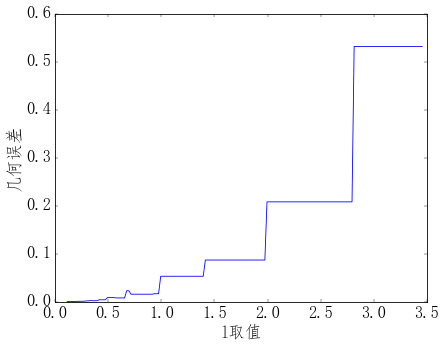
\includegraphics[width = \textwidth]{l-error0.png}
		\caption{$l$取值-子三角形质量关系图}\label{subfig:l-error0}
	\end{subfigure}%
	\begin{subfigure}[b]{.45\textwidth}
		\centering
		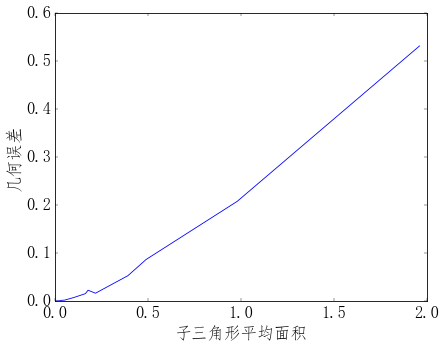
\includegraphics[width = \textwidth]{l-error1.png}
		\caption{子三角形数目-子三角形质量关系图}\label{subfig:l-error1}
	\end{subfigure}
	\caption{$l$取值-变形误差}\label{fig:l-error}
\end{figure}

\section{本章小结}
本章内容介绍了本文提出三角形均匀剖分算法的动机,用本文算法替换沿节点盒切割算法的可行性,本文算法的详细步骤以及本文算法的优势。除此之外,还讨论了三角形均匀剖分算法中参数$l$对于算法效率、剖分产生三角形的质量以及变形结果误差的影响。为用户选取合适的$l$提供了一定的指导。

% !TEX root = ../main.tex

\chapter{基于OpenGL Compute Shader实现算法}
CUDA是由英伟达推出的利用GPU进行通用计算的技术。该技术提供了方便易用的API,允许用户利用GPU强大的并行计算能力来加速算法,能得到了学术界和工业界的广泛应用。光滑自由变形\cite{Cui15}基于CUDA实现。大概获得了100多倍的加速。但是CUDA只能的在英伟达的硬件设备上运行,这大大限制了光滑自由变形的通用性,光滑自由变形不仅无法应用在其它的桌面平台的GPU(AMD、Intel核显)中,也无法在移动平台中运行。而后者由于计算资源有限,反而对GPU加速算法更加依赖。

所以,我们采用了OpenGL的Comput Shader实现本文算法,使得算法更加通用。在具体实现过程中,变形、微调三角贝赛尔曲面片(变形结果)的控制顶点,细分三角贝赛尔曲面片均采用和光滑自由变形相同的算法。不仅如此,我们还将光滑自由变形中CPU实现了部分——分割过程,实现在了GPU中,使整个算法都在GPU中完成。

\section{三角均匀剖分算法的GPU实现}
第\autoref{clip_algorithm}节中的算法是一个递归调用的算法,且算法中还有很多判断分支和特殊情况。


\section{引言}
三维模型形状编辑是图形学及其相关领域中不可或缺的一部分,无论在研究还是工业领域都存在着广泛的需求和应用。在经历了空间变形、多分辨率变形、微分域变形等几个研究热点之后,这一领域已得到了较为成熟的发展。众多研究者提出了各种方法以针对不同的需求场景。

但是随着网络带宽的增加,硬件性能的提升,使得大众可以很方便的传输、显示较大的三维模型。自然,大众对于模型质量的要求也随之提高,随之而来的还有对高质量三维内容的需求。另一方面,VR/AR的兴起进一步加强这一需求。这些也对三维模型形状编辑算法提出了新的要求,如提高编辑后模型的质量以满足大众对于高质量模型的需求,改进交互方式以便用户快速的创作三维模型,提升算法的效率使得用户可以编辑更大的模型。

空间变形作为一类简易,高效的三维模型形状编辑方法,近年来也发展出了一些新的变种以应对上文中提到的要求,如基于GPU的FFD算法\cite{chua2000, modat2010}、精确自由变形\cite{Feng98, Feng00}、光滑自由变形\cite{cui15}等。

本文的形容方向是自由变形,并在光滑自由变形\cite{cui15}的基础上提出了一种改进的算法。

光滑自由变形使用了CUDA加速算法,并根据模型的法向信息对变形结果进行了调整,使得算法具有实时编辑,变形结果更加自然细腻的优势。但是由于CUDA只能的Nvidia的显卡上运行,所以Cui的这一工作也被限制在了Nvidia平台上。另一方面,为了使组成模型的面片在变形后为贝赛尔三角片,光滑自由变形在预处理阶段需要将面片沿结点盒切割。该步骤很可能会产生一些狭长的或者退化的三角形,这些三角形不仅会造成计算资源的浪费,还可能影响算法的稳定性。

本文针对上述光滑自由变形的两个不足,进行了一系列深入的研究,在介绍本文工作之前,让我们先来回顾一下前人的相关工作。

\section{相关工作}
在诸多三维模型形状编辑算法中,空间变形是一种出现时间比较早,应用比较广泛的算法框架。该方案的基本思想最初由Barr\cite{Barr84}在1984年提出。Sederberg\cite{Sederberg86}于1986提出了经典的自由变形(Free-Form Deformation, 简称FFD),将这一思想完善为一个成熟的算法框架:
\begin{enumerate}
	\item 定义一个变形空间,也可以称之为中间体。
    \item 将待变形的模型“嵌入”到变形空间中,即计算模型上的采样点在变形空间中的参数坐标,该坐标在变形过程中保持不变。\label{item:2}
	\item 对变形空间进行变形。\label{item:3}
    \item 根据\ref{item:2}中得到的参数坐标与\ref{item:3}中得到的新变形空间,重新计算出采样点在欧氏空间中的坐标,从而达到变形的目的。
\end{enumerate}

\begin{figure}[htbp]
	\centering
	\begin{subfigure}[b]{.4\textwidth}
		\centering
		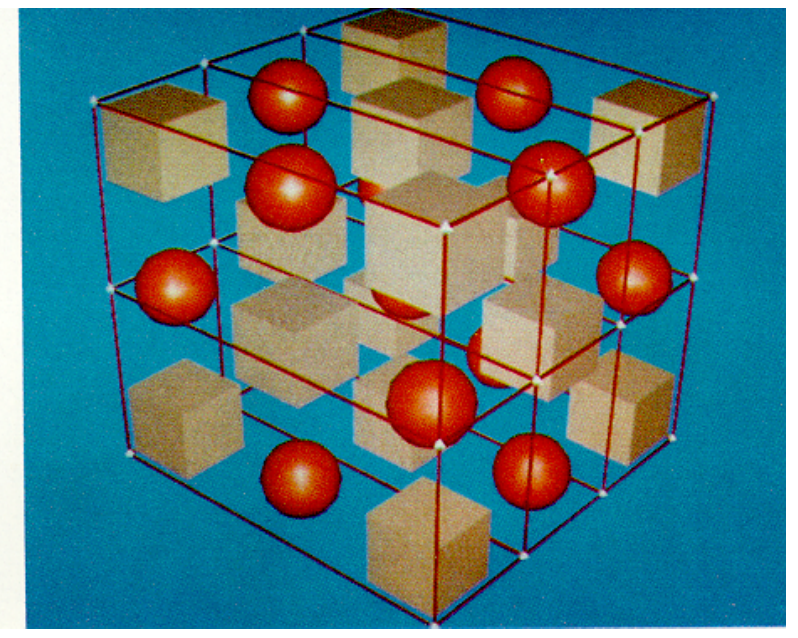
\includegraphics[width = \textwidth]{FFD_demo_0.png}
		\caption{原模型及中间体}\label{subfig:FFD_demo_0}
	\end{subfigure}
	\quad
	\begin{subfigure}[b]{.4\textwidth}
		\centering
		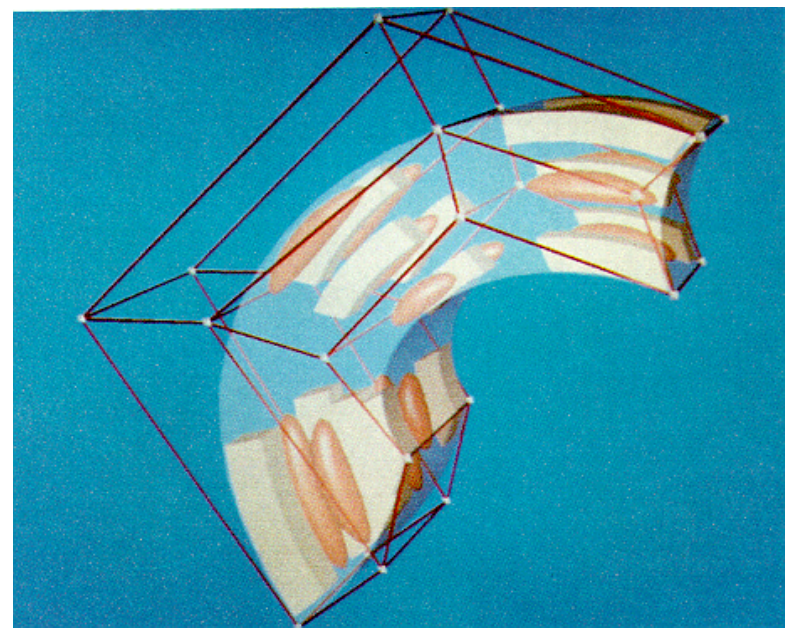
\includegraphics[width = \textwidth]{FFD_demo_1.png}
		\caption{FFD变形结果}\label{subfig:FFD_demo_1}
	\end{subfigure}
    \caption{自由变形示意图}\label{fig:FFD_demo}
\end{figure}

该方法具有直观、简单、高效的优点,很多学者在在此基础上提出了大量关于FFD算法的研究与改进。

中间体的选取是空间变形算法的关键,算法的效率、交互方式、变形结果等会因中间体表达方式的改变而改变。所以很多研究工作都着眼于中间体的改进:

Griessmair\cite{Griessmair89}和Lamousin\cite{lamousin1994}分别用B样条体和非均匀有理B样条体替换传统FFD\cite{Sederberg86}中的贝赛尔体,由于B样条体和非均匀有理B样条体的局部支撑性,使得模型的变形具有局部可调性。Coquillart\cite{coquillart1990}则通过移动、“焊接”长方体控制网格中的部分控制顶点,使得控制网格不再局限于长方体,而是将其转变圆柱等更加复杂的形状。这一改变虽然增加了变形模型嵌入变形空间过程中的计算量且对于控制网格的形状有一定的限制,但是改进了交互方式,使用户能够进行更为复杂的变形。

后续的学者进一步提出了以曲面、曲线甚至是以点为变形工具来构建变形空间。这些方法各自适用于不同的变形场合。如基于曲线的FFD适合基于骨架变形或者细长物体的变形,基于曲面的变形比较适用于形状较为扁平的模型的变形。总体而言,用户编辑模型时可以控制的变量越多,算法对模型的编辑能力就越强,能完成更加复杂的变形,但同时用户的交互也越复杂。在Gain和Beckmann的综述\cite{Gain08}中,作者对常见的FFD按照选用变形空间的不同进行了分类,并从局部可调性、交互友好度、时空效率、是否保拓扑等方面详细对比了各个方法的优劣。

上述这些方法中,无论中间体如何选择,用户都需要通过操作控制顶点来对中间体进行变形,中间体再通过采样点的参数坐标将变形“传导”到待变形的模型中。这一交互方式对普通用户而言并不友好,控制顶点的位移与待变形模型的顶点的位移并不完全一致。用户需对中间体的数学表示有所了解,才能实现复杂的变形意图。

为了解决这一问题,Hsu\cite{hsu1992}最先提出了直接自由变形,这一算法允许用户指定待变形模型上的一组点,并由用户提供这组点变形前后在欧氏空间中的位移。以前述信息为输入,算法将自动求出一组合适的控制顶点,使得用户指定的点的位移与输入保持一致。再由这组控制顶点求得最终变形结果。

随后,其它研究者也在此基础上提出了许多类似方法。这一类方法直接关联用户输入和变形结果,使用户直接编辑模型变形前后关键点的位置,即可等到整体的变形结果,而无需关心中间体的数学表示。使得FFD的交互更加便捷、直观。

传统FFD方法的另一个不足之处是变形过程中的走样问题。

由于传统FFd方法将变形是作用到待编辑模型的采样点上的,再由采样点变形后的位置,还原出模型的变形结果。所以,最终得到的变形结果的质量很大程度上依赖于采样点的密度。下\autoref{fig:sample_problem}很好的演示了这一问题。柜子的四个腿在原模型中由狭长的三角形组成,并且从视觉上看是与底部十字木条连在一起的。但是若以模型顶点为采样点,进行如\autoref{subfig:sample_problem_1}所示的变形后,柜子腿从视觉上与底部的十字木条分开了。这是由于采样点过于稀疏,变形只作用于柜子腿底部的顶点,而未作用于柜子腿与十字木条相连的部分造成的。

\begin{figure}[htbp]
	\centering
	\begin{subfigure}[b]{.4\textwidth}
		\centering
		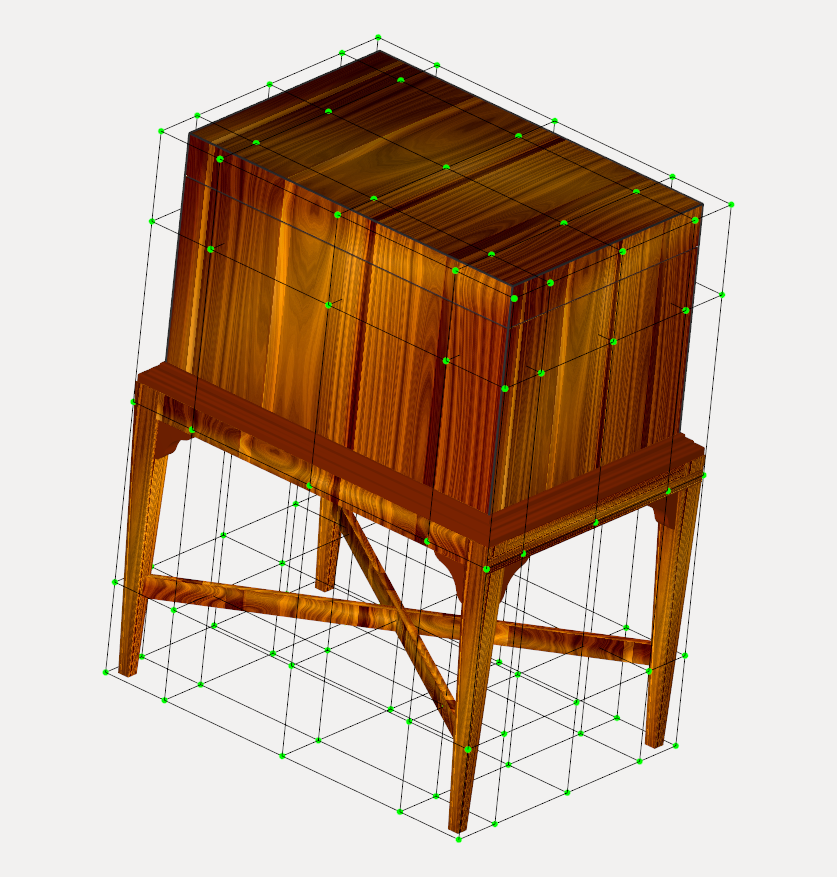
\includegraphics[width = \textwidth]{sample_problem_1.png}
		\caption{原模型}\label{subfig:sample_problem_0}
	\end{subfigure}
	\quad
	\begin{subfigure}[b]{.4\textwidth}
		\centering
		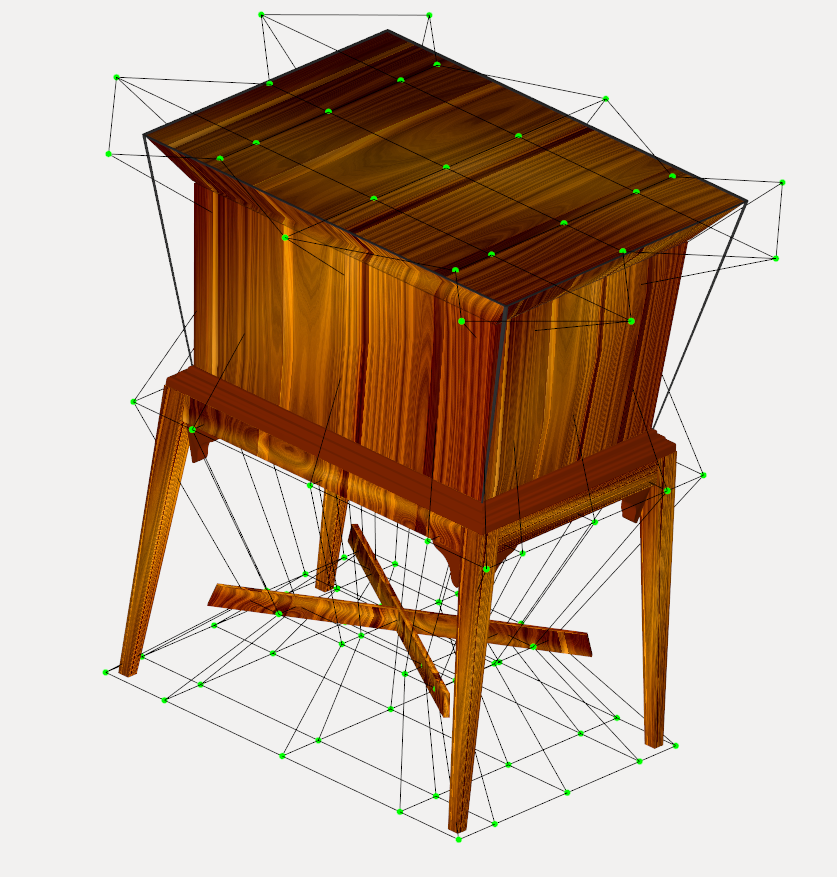
\includegraphics[width = \textwidth]{sample_problem_2.png}
		\caption{传统FFD变形结果}\label{subfig:sample_problem_1}
	\end{subfigure}
    \caption{传统FFD由于采样密度不足造成的精度问题}\label{fig:sample_problem}
\end{figure}

这一问题最直接的解决办法是通过均匀加密采样增加采样点的密度,但这一方法会造成性能上较大的开销。更进一步的方法\cite{parry1986, gain1999}是根据面片大小和曲面的曲率,自适应确定采样密度.自
适应采样虽然从性能上较之均匀加密采样有了较大的提升,但自适应算法实现相对复杂,并且无法很好的处理一些奇异情况。


为了更好的解决FFD中的走样问题,Feng\cite{Feng98}提出了“精确自由变形”。传统FFD是以采样点为变形对象的,而该方法以组成模型的曲面为变形对象的。变形算法的直接输出也不再是采样点变形后的位置,而是初始三角面片经由变形得到的新的曲面片。这样一来就避免了传统方法中采样过程所带来的走样问题。文中首先证明了:若自由变形采用的中间体为B样条体,且待变形的三角形位于B样条体某个节点盒之内,那么该三角形的变形结果为一个三角贝赛尔曲面片,且其次数为B样条体三个维度上的次数之和。然后,作者再通过函数复合\cite{derose1988, derose1993}和位移算子\cite{chang1984},计算出三角贝赛尔曲面片的控制顶点,从而得到精确而自然的变形结果。\autoref{fig:sample_problem_affd}中对比了精确FFD与传统FFD的变形结果。

\begin{figure}[htbp]
	\centering
	\begin{subfigure}[b]{.3\textwidth}
		\centering
		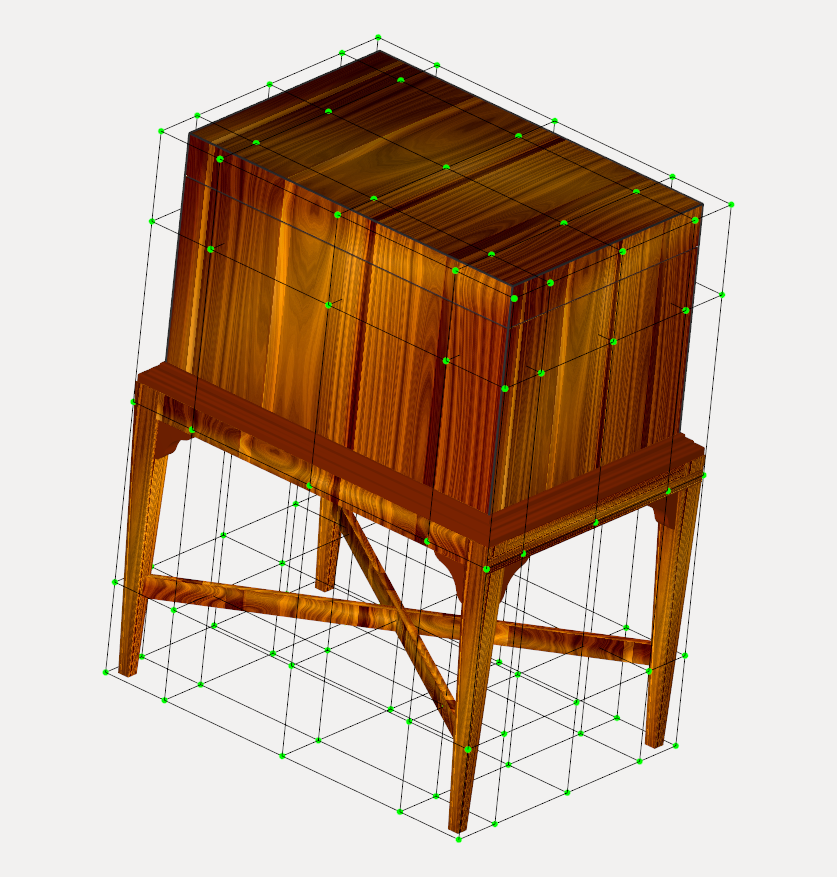
\includegraphics[width = \textwidth]{sample_problem_1.png}
		\caption{原模型}
	\end{subfigure}
	\quad
	\begin{subfigure}[b]{.3\textwidth}
		\centering
		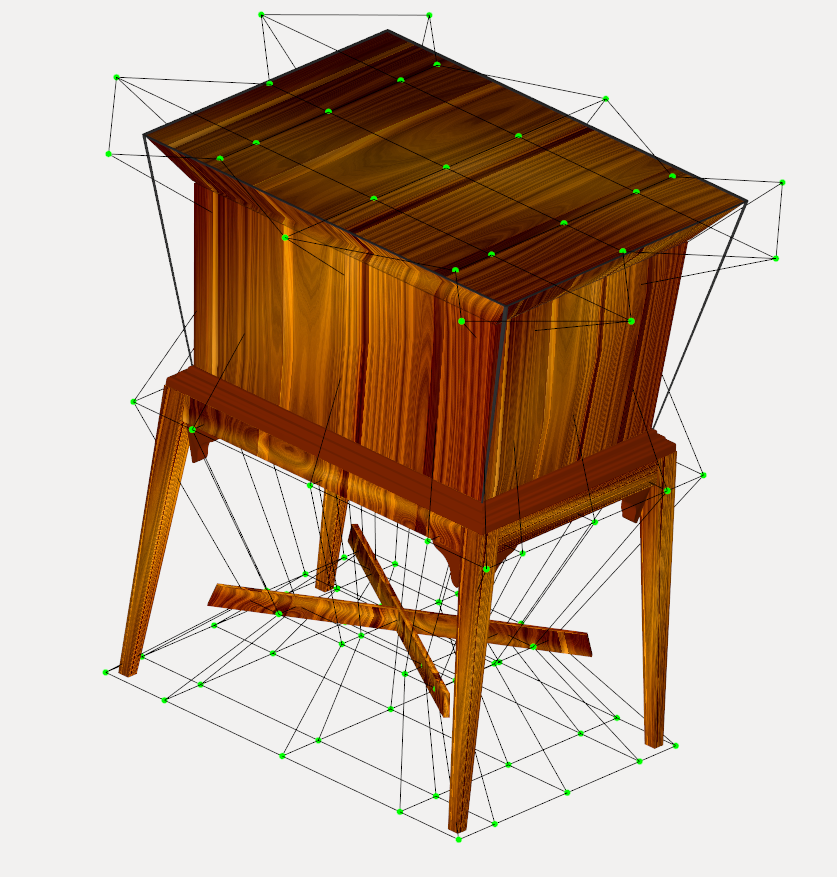
\includegraphics[width = \textwidth]{sample_problem_2.png}
		\caption{传统FFD变形结果}
	\end{subfigure}
	\quad
	\begin{subfigure}[b]{.3\textwidth}
		\centering
		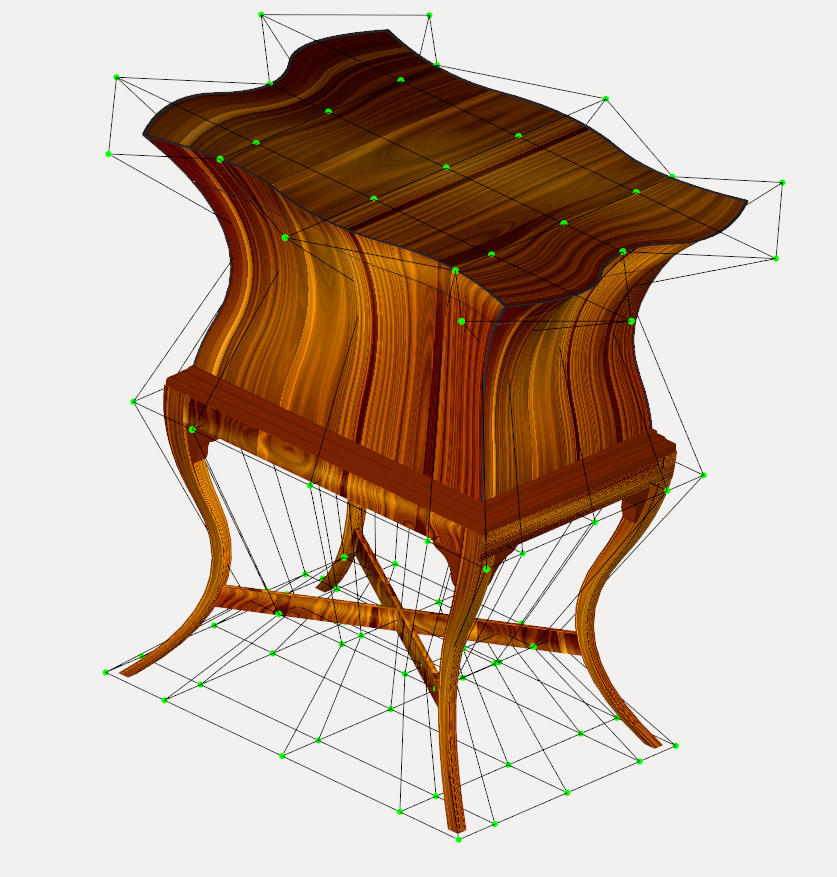
\includegraphics[width = \textwidth]{sample_problem_affd.png}
		\caption{精确FFD变形结果}
	\end{subfigure}
    \caption{传统FFD和精确FFD的结果对比}\label{fig:sample_problem_affd}
\end{figure}

作者在后续工作\cite{Feng00, Feng02}中对上述算法进行了改进,不仅使算法开销更低,还提升了算法的通用性。尽管如此,采用精确自由变形编辑较大的模型时,仍然无法做到实时交互。

另一方面,通用计算在近年来得到了较大的发展,GPU从一个仅负责图形绘制的专用硬件渐渐演变为一个多线程、高带宽的通用计算硬件。CUDA、OpenCL等通用计算框架的出现,更是进一步方便了应用程序利用GPU的强大的计算能力,以大幅提升其运行速度。FFD的构架下的算法大多是计算密集型的,且这些算法能较好的适用于单指令流多数据流计算模型,所以随着通用计算的兴起,自然有很多学者利用GPU加速各类FFD,从而使这些算法能对大型三维模型进行实时编辑。

其中,Cui\cite{Cui13}的工作成功地将CUDA应用到了精确自由变形中,采用GPU实现的算法相较于原先的CPU版本快了50倍左右。另一方面,无论是传统的FFD还是精确FFD,在其变形过程中都只考虑了待变形的模型的几何信息,而未考虑模型的法向信息。所以变形之后得到的模型会有不光滑的走样,\autoref{subfig:saffd_0}和\autoref{subfig:saffd_1}演示了这种走样现象。为了解决这些问题,Cui在其后续工作\cite{cui15}中提出了光滑自由变形。在精确自由变形的基础上,光滑自由变形根据法向信息对变形后得到的曲面片进行了微调,以得到如\autoref{subfig:saffd_2}所示的光滑外观。

\begin{figure}[htbp]
	\centering
	\begin{subfigure}[b]{.3\textwidth}
		\centering
		\includegraphics[width = \textwidth]{saffd_0.png}
		\caption{传统自由变形结果}\label{subfig:saffd_0}
	\end{subfigure}
	\quad
	\begin{subfigure}[b]{.3\textwidth}
		\centering
		\includegraphics[width = \textwidth]{saffd_1.png}
		\caption{精确自由变形结果}\label{subfig:saffd_1}
	\end{subfigure}
	\quad
	\begin{subfigure}[b]{.3\textwidth}
		\centering
		\includegraphics[width = \textwidth]{saffd_2.png}
		\caption{光滑自由变形结果}\label{subfig:saffd_2}
	\end{subfigure}
    \caption{传统自由变形、精确自由变形和光滑自由变形的结果对比}\label{fig:sample_problem_affd}
\end{figure}


%自由变形(Free Form Deformation)是一类编辑几何模型、生成柔体性动画的方法。由于其实现简单,与模型表示无关,所以被广泛的应用于计算机辅助设计与工程、计算机动画、医学影影等领域。另一方面,由于其较强的可拓展性,FFD\cite{Sederberg86}自提出以来就受到了学术届的广泛关注,该工作不仅实现了一种具体的编辑三维模型的方法,更重要的是是提出了一套编辑三维模型的算法框架。研究人员在这一框架的基础上,做了很多工作。主要从算法效率、变形结果、交互方式三方面对FFD进行了改进:


%在FFD交互方式的探索中,研究者主要着眼于变形空间的选取。不同的变形空间,适用于不同的编辑需求,同时也会影响用户的交互方式。总体而言,用户编辑模型时可以控制的变量越多,算法对模型的编辑能力就越强,同时用户的交互也越复杂。


\section{本文内容安排}
本文的内容安排如下:

\section{引言}
以下是一个测试用的列表环境,内容不要在意。\footnote{正文中中脚注命令测试,长脚注情况:这包括如下事实:“未经本人同意,监听、录制或转播私人性质的谈话或秘密谈话;未经本人同意,拍摄、录制或转播个人在私人场所的形象”}

这里测试列表标签功能的交叉引用格式\ref{itm:11},\ref{itm:12},\ref{itm:13},\ref{itm:14},分别表示第一至第四层级的itemize系列的交叉引用情况。
\begin{enumerate}
	\item 第一级列表\label{itm:11}
	\begin{enumerate}
		\item 第二级列表\label{itm:12}
	\end{enumerate}
\end{enumerate}

\begin{itemize}
	\item 第一级列表
	\begin{itemize}
		\item 第二级列表
	\end{itemize}
\end{itemize}

\section{浮动体测试}
\subsection{插图测试}
如\autoref{fig:first_image_tset}是对此模版的第一张插图测试。

\begin{figure}[htbp]
	\centering
	\includegraphics[width = 0.5\linewidth]{Chapter1.png}
	\caption{第一张插图测试}\label{fig:first_image_tset}
\end{figure}

\subsection{表格测试}

\subsubsection{array宏包tabular表格环境测试}
如\autoref{tab:first_table_test}是对array宏包的tabular表格环境测试。
\begin{table}[htbp]
	\centering
	\caption{这是一个用tabular环境的测试用的表格}\label{tab:first_table_test}
    \begin{tabular}{lrr}
    \toprule
    \textbf{行星}     & \textbf{赤道半径}km & \textbf{公转周期}d \\
    \midrule
    水星     & 2.439  & 87.9 \\
    金星     & 6.1    & 224.682 \\
    地球     & 6378.14 & 365.24 \\
    \bottomrule
    \end{tabular}%
\end{table}

\subsubsection{tabu宏包表格环境测试}
如\autoref{tab:tabu_test_1}是对tabu宏包的tabu表格环境测试。在这里表格命令与\autoref{tab:first_table_test}的命令相同,只是tabular环境改成了tabu环境。
\begin{table}[htbp]
	\centering
	\caption{这是一个用tabu环境的测试用的表格}\label{tab:tabu_test_1}
    \begin{tabu}{lrr}
    \toprule
    \textbf{行星}     & \textbf{赤道半径}km & \textbf{公转周期}d \\
    \midrule
    水星     & 2.439  & 87.9 \\
    金星     & 6.1    & 224.682 \\
    地球     & 6378.14 & 365.24 \\
    \bottomrule
    \end{tabu}%
\end{table}

\autoref{tab:tabu_test_2}对tabu to表格的x列模式进行测试。在表格导言区中设置为X[1]X[2]X[2],表示这三列表格的列宽比值为1:2:2,总的表格宽度由tabu to环境设置,这里设置为0.6\textbackslash linewidth。相比于tabular环境,tabu环境的列宽设置方便许多。
\begin{table}[htbp]
	\centering
	\caption{tabu环境测试表格---X列模式}\label{tab:tabu_test_2}
    \begin{tabu} to 0.6\linewidth{X[1]X[2]X[2]}
    \toprule
    \textbf{行星}     & \textbf{赤道半径}km & \textbf{公转周期}d \\
    \midrule
    水星     & 2.439  & 87.9 \\
    金星     & 6.1    & 224.682 \\
    地球     & 6378.14 & 365.24 \\
    \bottomrule
    \end{tabu}%
\end{table}

特别需要注意的是,longtabu是基于longtable宏包开发的,所以在zjuthesis.cls文件中已经插入了longtable宏包。longtable环境的所有功能都可以在longtabu中使用,如\textbackslash endhead,\textbackslash endfirsthead,\textbackslash endfoot,\textbackslash endlastfoot,和\textbackslash caption等。具体用法请参见longtable和tabu宏包的相应文档。
\begin{longtabu}{lccc}
\caption{材料弹性模量及泊松比}\label{tab:tabu_test_3}\\
\toprule
名  称   & 弹性模量E/Gpa & 切变模量G/Gpa & 泊松比$\mu$ \\
\midrule%
\endfirsthead
\caption{材料弹性模量及泊松比(续)}\\
\toprule
名  称   & 弹性模量E/Gpa & 切变模量G/Gpa & 泊松比$\mu$ \\
\midrule%
\endhead
\bottomrule%
\endfoot
镍铬钢、合金钢 & 206    & 79.38  & 0.3 \\
碳 钢    &  196~206 & 79     & 0.3 \\
\end{longtabu}%

\subsection{子图}

如\autoref{fig:subfig_test1}是有两张子图的模式,对子图进行交叉引用,如\autoref{subfig:1a}和\autoref{subfig:1b}。

\begin{figure}[htbp]
	\centering
	\begin{subfigure}[b]{.4\textwidth}
		\centering
		\includegraphics[width = \textwidth]{Chapter2.png}
		\caption{书籍排版与普通排版}\label{subfig:1a}
	\end{subfigure}
	\quad
	\begin{subfigure}[b]{.4\textwidth}
		\centering
		\includegraphics[width = \textwidth]{Chapter3.png}
		\caption{\TeX 的控制系列}\label{subfig:1b}
	\end{subfigure}
	\caption{子图模式测试1:2张图}\label{fig:subfig_test1}
\end{figure}

\begin{figure}[htbp]
	\centering
	\begin{subfigure}[b]{.4\textwidth}
		\centering
		\includegraphics[width = \textwidth]{Chapter4.png}
		\caption{字体}\label{subfig:2a}
	\end{subfigure}
	\begin{subfigure}[b]{.4\textwidth}
		\centering
		\includegraphics[width = \textwidth]{Chapter5.png}
		\caption{编组}\label{subfig:2b}
	\end{subfigure}
	\begin{subfigure}[b]{.4\textwidth}
		\centering
		\includegraphics[width = \textwidth]{Chapter6.png}
		\caption{运行\TeX}\label{subfig:2c}
	\end{subfigure}
	\begin{subfigure}[b]{.4\textwidth}
		\centering
		\includegraphics[width = \textwidth]{Chapter7.png}
		\caption{\TeX 工作原理}\label{subfig:2d}
	\end{subfigure}
	\caption{子图模式测试2:4张图}\label{fig:subfig_test2}
\end{figure}

\subsection{数学模式测试}
数学模式测试,主要测试数学字体,编号和交叉引用。这里首先推荐使用\texttt{align}和\texttt{align*}数学模式环境,大多数行间数学模式只需要用这个环境就可以了。

交叉引用测试,如交引用命令{\ttfamily \textbackslash eqref}和\texttt{\textbackslash ref}命令的区别。如公式\eqref{eq:test1},公式\ref{eq:test1}显示,\texttt{\textbackslash eqref}命令比\texttt{\textbackslash ref}命令的应用结果多了个括号。

如公式\eqref{eq:test3}是单行公式环境,查看公式\eqref{eq:test3}和\eqref{eq:test1}之间的区别,好像在单行公式中没什么区别。
\begin{align}\label{eq:test3}
	f(x) = 2(x + 1)^{2} - 1
\end{align}

\texttt{align}公式环境,用在单行中。
\begin{align}\label{eq:test1}
	f(x) = 2(x + 1)^{2} - 1
\end{align}

\begin{align*}
	f(x) = 2(x + 1)^{2} - 1
\end{align*}
在这里,中间插入一些文字以形成段落,查看行间公式与上下文之间的间隙。下一个公式\eqref{eq:test2}是一个公式组,它在“=”位置对齐。
\begin{align}\label{eq:test2}
	f(x) & = 2(x + 1)^{2} - 1\\
		 & = 2(x^{2} + 2x +1)-1\\
		 & = 2x^{2} + 4x + 1
\end{align}


\section{关于引用}
图表的引用通过{\ttfamily \textbackslash autoref} 命令即可,使用ST LaTeXTools 插件还能自动补全。如果要修改前缀,那么就用{\ttfamily \textbackslash recnewcommand \textbackslash figureautorefname\{好图\}}即可,详见hyperref宏包说明。

% !TEX root = ../main.tex
\chapter{算法在移动平台的实现}
本文方法用OpenGL Compute Shader实现,所以理论上可以在任何支持OpenGL 4.3的设备上运行。为了验证这一点,我们将本文方法应用到了哇陶中。哇陶是一个安卓平台上的陶瓷制作过程模拟软件。用户可以借助该软件体验陶瓷制作全过程\footnote{不同的瓷器,制作步骤会有所区别。哇陶中的过程与常用的青花瓷制作过程保持一致:泥胚塑形、烧制、贴花。},如\autoref{哇陶图片}所示。如果用户对自己制作的瓷器感到很满意,还可以下单购买。

% todo 哇陶图片。

在真实的陶瓷制作过程中,泥胚塑形阶段制作陶瓷的工匠不仅可以通过转台将瓷器拉成一个旋转体,还可以通过捏胚将瓷器塑造成任意形状。其中拉胚过程在软件中较容易模拟,略过不述。但是捏胚的过程是一个典型的三维模型形状编辑过程。本文方法应用于此以帮助用户得到满意的造型。




移动设备中实现。我们将该方法应用到了一款安卓软件\footnote{哇陶是一款陶瓷制作过程模拟软件,用户可以借助该软件参与到陶瓷制作的各个过程中(拉胚、烧制、贴花等)。}中,使得用户可以在拉胚阶段自由的编辑瓷器形状。


% !TEX root = ../main.tex
\chapter{结果对比}
本章主要进行了绘制效果,算法效率,算法精度这三方面的对比,我们进行对比实验的硬件条件如下:CPU为英特尔酷睿i7 4710MQ@2.50GHz,GPU为英伟达GeForce GT 730M,内存大小为8GB。对比的对象是传统的自由变形\cite{Sederberg86}和光滑自由变形\cite{Cui15}。选用的变形空间均为B样条体,其次数为$3\times3\times3$,控制顶点个数为$6\times6\times6$。为了方便比较,待变形的模型顶点都将先归一化到$[-1, 1]^3$

由于光滑自由变形和本文算法最终的变形结果均为三角Bézier曲面片,本文采取与光滑自由变形相同的方案可视化这些曲面片,即均匀细分成三角形然后通过OpenGL绘制。用户可以通过参数控制三角Bézier曲面片的细分粒度,以将解析结果细分成不同精度的三角网格模型。在本章的实验中,所有三角Bézier曲面片都将被均匀细分成100个小三角形进行绘制。同时在比较光滑自由变形和本文方法的拟合误差时,误差值也将通过比较细分后三角形顶点的属性得到的。

在以下对比实验中,本文方法在分割阶段时,$l$的值固定为$\frac{1}{3}$的节点盒长度。

\section{绘制效果比对}
本节主要对比传统自由变形、光滑自由变形以及本文算法的绘制效果。对比实验的硬件环境与算法参数如上文所述。实验中选用帆船作为对比模型,该模型中包含了各种大小、各种形状的三角形,能够有效的检验变形算法产生结果的质量。

\autoref{subfig:renderer_effect}中展示了各个方法的绘制结果,\autoref{subfig:renderer_effect1}是传统自由变形的结果,可以很明显的看到帆船桅杆部分因采样密度不足造成的走样问题。光滑自由变形(\autoref{subfig:renderer_effect3})和本文方法(\autoref{subfig:renderer_effect2})均很好的解决了这一问题。

同时通过比较\autoref{subfig:renderer_effect3}和\autoref{subfig:renderer_effect2},可以发现本文算法和光滑自由变形的结果,从视觉上基本无法区分。\autoref{subfig:renderer_effect4}是本文方法和光滑自由变形的像素层面上的差异。红色的深度越深表示差异越大。白色表示没有差异。\autoref{subfig:renderer_effect3}和\autoref{subfig:renderer_effect2}的像素用256阶灰度表示,除去背景像素,两者像素值平均差异是$0.249$,最大差异是$51$。其中灰度差异小于5的像素点了占了总像素点的$99.02\%$。所以肉眼几乎无法看出两者差别。

通过以上分析,可以认为本文方法达到了和光滑自由变形相同的绘制效果。
\begin{figure}[htbp]
	\centering
	\begin{subfigure}[b]{.4\textwidth}
		\centering
		\includegraphics[width = \textwidth]{renderer_effect0.png}
		\caption{原始模型}\label{subfig:renderer_effect0}
	\end{subfigure}
	\quad
	\begin{subfigure}[b]{.4\textwidth}
		\centering
		\includegraphics[width = \textwidth]{renderer_effect1.png}
		\caption{传统自由变形结果}\label{subfig:renderer_effect1}
	\end{subfigure}

	\centering
	\begin{subfigure}[b]{.4\textwidth}
		\centering
		\includegraphics[width = \textwidth]{renderer_effect3.png}
		\caption{光滑变形结果}\label{subfig:renderer_effect3}
	\end{subfigure}
	\quad
	\begin{subfigure}[b]{.4\textwidth}
		\centering
		\includegraphics[width = \textwidth]{renderer_effect2.png}
		\caption{本文方法结果}\label{subfig:renderer_effect2}
	\end{subfigure}

	\centering
	\begin{subfigure}[b]{.4\textwidth}
		\centering
		\includegraphics[width = \textwidth]{renderer_effect4.png}
        \caption{\autoref{subfig:renderer_effect3}和\autoref{subfig:renderer_effect2}的像素差异}\label{subfig:renderer_effect4}
	\end{subfigure}
	\quad
	\begin{subfigure}[b]{.4\textwidth}
		\centering
		\includegraphics[width = \textwidth]{renderer_effect5.png}
		\caption{带纹理的本文结果}\label{subfig:renderer_effect5}
	\end{subfigure}
	\caption{绘制效果对比图}\label{subfig:renderer_effect}
\end{figure}

\section{效率对比}
本节的比较的对象仍然是光滑自由变形,选用的模型是一个高精度的蜗牛模型,如\autoref{fig:speed_compare}所示,由46742个面片组成。

\begin{figure}[htbp]
	\centering
	\begin{subfigure}[b]{.4\textwidth}
		\centering
		\includegraphics[width = \textwidth]{snail1.png}
		\caption{光滑自由变形绘制结果}\label{subfig:snail1}
	\end{subfigure}
	\quad
	\begin{subfigure}[b]{.4\textwidth}
		\centering
		\includegraphics[width = \textwidth]{snail2.png}
		\caption{本文方法绘制结果}\label{subfig:snail2}
	\end{subfigure}
	\caption{效率对比采用的蜗牛模型}\label{fig:speed_compare}
\end{figure}

\subsection{分割阶段}
光滑自由变形的分割阶段在CPU中完成,本文方法在GPU中完成。\autoref{tab:clip_time_compare}中是两种方法在分割阶段所用的时间,本文方法具有较大优势,速度上快了近200倍。这其中在两方面的原因,一方面我们通过以空间换时间的策略,对较为耗时的“计算分割方案”这一过程进行了预计算。另一方面是我们用GPU实现了分割过程,而光滑自由变形是在CPU中实现的。

\begin{table}[htbp]
    \centering
    \caption{三角形分割阶段运行时间对比(单位:ms)}\label{tab:clip_time_compare}
    \begin{tabular}{lrr}
    \toprule
    \textbf{步骤}   & \textbf{本文方法} & \textbf{光滑自由变形\cite{Cui15}} \\
    \midrule
    生成PN三角形    & 4.618             & 104.465                           \\
    切割原始三角面片& 21.475            & 5027.418                          \\
    \midrule
    \textbf{总计}   & 26.093            & 5131.883                          \\
    \bottomrule
    \end{tabular}
\end{table}

\subsection{变形、绘制阶段}
变形过程又分为几个以下几个子过程:
\begin{enumerate}
    \item 计算拟合点。
    \item 计算约束点。
    \item 计算三角Bézier曲面片的控制顶点。
    \item 调整控制顶点。
\end{enumerate}

绘制也可以分为两个子过程:
\begin{enumerate}
    \item 离散化三角Bézier曲面片。
    \item 绘制。
\end{enumerate}

其中,绘制交由OpenGL流水管线实现,故不比较这一过程的时间。其它过程计算时间如\autoref{tab:deformation_time_compare}所示。

\begin{table}[htbp]
    \centering
    \caption{三角形变形、绘制阶段运行时间对比(单位:ms)}\label{tab:deformation_time_compare}
    \begin{tabular}{lrr}
    \toprule
    \textbf{步骤}     & \textbf{本文方法} & \textbf{光滑自由变形\cite{Cui15}} \\
    \midrule
    计算采样点位置     & \multirow{6}{*}{67.419} & 41.369     \\
    计算三角Bézier曲面片控制顶点      &                         & 11.125     \\
    计算三角Bézier曲面片的法向量场   &                         & 4.209     \\
    微调控制顶点         &                         & 4.344     \\
    离散三角Bézier曲面片 &                         & 4.057     \\
    \midrule
    \textbf{总计}& 67.419  & 65.464    \\
    \bottomrule
    \end{tabular}
\end{table}
本文采用OpenGL Compute Shader实现,为了尽可能提高运行效率,\autoref{tab:deformation_time_compare}中的几个阶段实现在了同一个Shader中,所以以上几个阶段本文方法只给出了总运行时间。

光滑自由变形由CUDA实现,该方法在实现上述过程时,大量的采用了大矩阵乘法,并交由cuBLAS计算。cuBLAS是CUDA官方提供的线性运算库,在相同的硬件下,实现相同的计数任务,用户自己编写的程序很难在时间效率上超过cuBLAS。所以我们有理由将光滑自由变形的变形过程所用的时间作为一个性能的标杆。本文以之为目标,作了很多算法及语言层面上的优化。最终得到的结果只比光滑自由变形慢了$2.99\%$。考虑到我们的算法采用的OpenGL Compute Shader实现,OpenGL Compute Shader并末提供大矩阵运算库,无法从大矩阵运算中得益,所以我们认为本文变形所用的时间是一个较为合理的结果。

\subsection{总结}
综上所述,在变形、绘制阶段,本文算法基本能达到和光滑自由变形相同的运行速度。而在分割阶段,本文方法具有较大优势,约比光滑自由变形快了近200倍。

\section{精度对比}
虽然光滑自由变形基于精确自由变形,但是该方法最终变形结果是通过用低次的三角Bézier曲面片拟合高次的精确结果得到,这样虽然提高了算法的运行效率,但同时也引入了法向和几何上的误差。本文方法也存在相同的拟合误差,并且本文未沿节点盒切割原始三角面片,这也是一个误差增加的潜在因素。本节希望通过误差分析说明本文方法的误差相较于自由变形并不会有显著增加。

本节中,本文方法的比较对象仍是光滑自由变形,我们分别计算光滑自由变形、本文方法的变形结果与精确结果的差异以得到两种方法对应的误差值。与光滑自由变形一样,本文方法也会通过法向信息微调三角Bézier曲面片的控制顶点。所以我们需要几何与法向都精确的模型作为本节实验变形所用的模型。为此我们选择了一个标准的立方体和一个由36个三次Bézier曲面组成的Utah茶壶作为变形模型进行误差分析,如\autoref{fig:error_ori}所示。标准立方体的精确变形结果可以通过精确自由变形\cite{Feng00}得到,Utah茶壶的精确变形结果可以通过传统FFD结合均匀加密采样得到。由于Utah茶壶是由Bézier曲面片组成的,所以必须先转化成多边形网格才能作为变形算法的输入,我们采用Casteljau细分算法\cite{farin2000essentials}将其转化成多边形网格。

\begin{figure}[htbp]
	\centering
	\begin{subfigure}[b]{.4\textwidth}
		\centering
		\includegraphics[width = \textwidth]{cube0.png}
		\caption{立方体}\label{subfig:cube0}
	\end{subfigure}
	\quad
	\begin{subfigure}[b]{.4\textwidth}
		\centering
		\includegraphics[width = \textwidth]{teapot0.png}
		\caption{Utah茶壶}\label{subfig:teapot0}
	\end{subfigure}
	\quad
	\caption{误差估计采用的模型}\label{fig:error_ori}
\end{figure}

\autoref{fig:cube_result}和\autoref{fig:teapot_result}是分别是立方体和Utah茶壶的在各个变形方法下的变形结果。

\begin{figure}[htbp]
	\centering
	\begin{subfigure}[b]{.3\textwidth}
		\centering
		\includegraphics[width = \textwidth]{cube1.png}
		\caption{精确自由变形结果}\label{subfig:cube1}
	\end{subfigure}
	\begin{subfigure}[b]{.3\textwidth}
		\centering
		\includegraphics[width = \textwidth]{cube2.png}
		\caption{光滑自由变形结果}\label{subfig:cube2}
	\end{subfigure}
	\begin{subfigure}[b]{.3\textwidth}
		\centering
		\includegraphics[width = \textwidth]{cube3.png}
		\caption{本文结果}\label{subfig:cube3}
	\end{subfigure}
	\caption{立方体变形结果}\label{fig:cube_result}
\end{figure}

\begin{figure}[htbp]
	\centering
	\begin{subfigure}[b]{.3\textwidth}
		\centering
		\includegraphics[width = \textwidth]{teapot1.png}
		\caption{传统自由变形结果}\label{subfig:teapot1}
	\end{subfigure}
	\begin{subfigure}[b]{.3\textwidth}
		\centering
		\includegraphics[width = \textwidth]{teapot2.png}
		\caption{光滑自由变形结果}\label{subfig:teapot2}
	\end{subfigure}
	\begin{subfigure}[b]{.3\textwidth}
		\centering
		\includegraphics[width = \textwidth]{teapot3.png}
		\caption{本文结果}\label{subfig:teapot3}
	\end{subfigure}
	\caption{Utah茶壶变形结果}\label{fig:teapot_result}
\end{figure}

\autoref{subfig:cube1}是立方体模型通过精确自由变形得到的结果,该结果是精确的,所以光滑自由变形和本文方法得到的结果(如图\autoref{subfig:cube2}与\autoref{subfig:cube3}所示)都与精确自由变形得到的结果进行比较,以得到两者的变形误差,结果如\autoref{tab:error_cube}所示。其中,几何误差定义为对应点的欧氏距离,法向误差定义为对应点法向所成夹角的角度。从\autoref{tab:error_cube}中可以看出,本文方法的几何误差与法向误差均小于光滑自由变形,主要原因是本文方法选取的$l$比较小,产生的子三角形要比光滑自由变形小很多。\autoref{fig:cube_error0}、\autoref{fig:cube_error1}中是上述误差的可视化结果。

\begin{table}[htbp]
    \centering
    \caption{立方体误差} \label{tab:error_cube}
    \begin{tabular}{lrrrr}
    \toprule
                    & 平均几何误差 & 最大几何误差 & 平均法向误差 & 最大法向误差 \\
    \midrule
        本文方法    & \num{0.002952310} & \num{0.02908119} & \num[scientific-notation=false]{0.5785680}$^\circ$ & \num[scientific-notation=false]{15.89719}$^\circ$ \\
        光滑自由变形& \num{0.004904391} & \num{0.03718415} & \num[scientific-notation=false]{0.5853341}$^\circ$ & \num[scientific-notation=false]{21.24638}$^\circ$ \\
    \bottomrule
    \end{tabular}
\end{table}

\begin{figure}[htbp]
	\centering
	\begin{subfigure}[b]{.45\textwidth}
		\centering
		\includegraphics[width = \textwidth]{cube4.png}
		\caption{本文方法几何误差图}\label{subfig:cube4}
	\end{subfigure}%
	\begin{subfigure}[b]{.45\textwidth}
		\centering
		\includegraphics[width = \textwidth]{cube6.png}
		\caption{光滑自由变形几何误差图}\label{subfig:cube6}
	\end{subfigure}
	\caption{立方体几何误差}\label{fig:cube_error0}
\end{figure}
\begin{figure}[htbp]
	\centering
	\begin{subfigure}[b]{.45\textwidth}
		\centering
		\includegraphics[width = \textwidth]{cube5.png}
		\caption{本文方法法向误差图}\label{subfig:cube5}
	\end{subfigure}%
	\begin{subfigure}[b]{.45\textwidth}
		\centering
		\includegraphics[width = \textwidth]{cube7.png}
		\caption{光滑自由变形法向误差图}\label{subfig:cube7}
	\end{subfigure}
	\caption{立方体法向误差}\label{fig:cube_error1}
\end{figure}

对于Utah茶壶,对比结果如\autoref{tab:error_utah}所示。我们同样给出了上述误差的可视化结果,如\autoref{fig:teapot_error0}、\autoref{fig:teapot_error1}所示。Utah茶壶经过Casteljau细分算法得到的三角形本身比较小,因此本文方法中较小的$l$没有优势,所以两种结果的几何误差和法向误差较为接近。同时从\autoref{subfig:teapot5}和\autoref{subfig:teapot7}可以看出,无论上本文方法还是光滑自由变形,曲率较大的地方法向误差都会比较大。

\begin{table}[htbp]
    \centering
    \caption{Utah茶壶误差} \label{tab:error_utah}
    \begin{tabular}{lrrrr}
    \toprule
        & 平均几何误差 & 最大几何误差 & 平均法向误差 & 最大法向误差 \\
    \midrule
        本文方法    & \num{0.006597950} & \num{0.01203453} & \num[scientific-notation=false]{0.6152188}$^\circ$ & \num[scientific-notation=false]{22.53011}$^\circ$ \\
        光滑自由变形& \num{0.006650957} & \num{0.01220984} & \num[scientific-notation=false]{0.5491496}$^\circ$ & \num[scientific-notation=false]{22.53010}$^\circ$ \\
    \bottomrule
    \end{tabular}
\end{table}

\begin{figure}[htbp]
	\centering
	\begin{subfigure}[b]{.45\textwidth}
		\centering
		\includegraphics[width = \textwidth]{teapot4.png}
		\caption{本文方法几何误差图}\label{subfig:teapot4}
	\end{subfigure}%
	\begin{subfigure}[b]{.45\textwidth}
		\centering
		\includegraphics[width = \textwidth]{teapot6.png}
		\caption{光滑自由变形几何误差图}\label{subfig:teapot6}
	\end{subfigure}
	\caption{Utah茶壶几何误差}\label{fig:teapot_error0}
\end{figure}
\begin{figure}[htbp]
	\centering
	\begin{subfigure}[b]{.45\textwidth}
		\centering
		\includegraphics[width = \textwidth]{teapot5.png}
		\caption{本文方法法向误差图}\label{subfig:teapot5}
	\end{subfigure}%
	\begin{subfigure}[b]{.45\textwidth}
		\centering
		\includegraphics[width = \textwidth]{teapot7.png}
		\caption{光滑自由变形法向误差图}\label{subfig:teapot7}
	\end{subfigure}
	\caption{Utah茶壶法向误差}\label{fig:teapot_error1}
\end{figure}

%% !TEX root = ../main.tex
\chapter{学位论文基本结构}
学位论文基本结构包括前置部份、主体部份和结尾部份\footnote{测试脚注另起一章编号的变化}。
\section{前置部分包括}
\begin{enumerate}
	\item 封面
	\item 题名页
	\item 英文题名页(硕士可省略)
	\item 独创性声明(知识产权声明?)
	\item 勘误表(可根据需要)
	\item 致谢
	\item 序言或前沿(可根据需要)
	\item 摘要页
	\item 目次页
	\item 插图和附表清单(可根据需要)
	\item 缩写、符号清单、术语表(可根据需要)
\end{enumerate}
\section{主体部分}
\begin{enumerate}
	\item 引言(绪论)
	\item 正文
	\item 结论
\end{enumerate}
\section{结尾部分}
\begin{enumerate}
	\item 参考文献
	\item 附录(可根据需要)
	\item 索引(根据需要)
	\item 作者简历及在学期间所取得的科研成果
	\item 封底
\end{enumerate}
\chapter{版面设置}
\section{字体设置}
字体设置
\begin{table}[htb]
	\caption{文章字体设置效果}
	\label{tab:文章字体设置效果}
	\begin{center}
		\begin{tabular}{ccc}
			\toprule
					& 英文字体 & 中文字体  \\
			\midrule
			正文字体 & I can eat glass, it doesn't hurt me. & 我能吞下玻璃而不伤身体 \\
			\textbackslash textrm\{\} & \textrm{I can eat glass, it doesn't hurt me.} & \textrm{我能吞下玻璃而不伤身体} \\
			\textbackslash textsf\{\} & \textsf{I can eat glass.} & \textsf{我能吞下玻璃而不伤身体} \\
			\textbackslash texttt\{\} & \texttt{I can eat glass.} & \texttt{我能吞下玻璃而不伤身体} \\
			\textbackslash textbf\{\} & \textbf{I can eat glass.} & \textbf{我能吞下玻璃而不伤身体} \\
			\bottomrule
		\end{tabular}
	\end{center}
\end{table}

%% !TEX root = ../main.tex
\chapter{编写规范与要求}
\section{前置部分}
\subsection{封面}
封面包括分类号、密级、单位代码、作者学号、校名、学校徽标、学位论文中文题目、英文题目、作者姓名、导师姓名、学科和专业名称、提交时间等内容(\textbf{见附件1:学位论文封面样式})。
\subparagraph{分类号} % (fold)
\label{par:分类号}
按中国图书分类法,根据学位论文的研究内容确定。
% subparagraph 分类号 (end)
\subparagraph{密级} % (fold)
\label{par:密级}
仅限于涉密学位论文(论文课题来源于国防军工项目)填写,密级应根据涉密学位论文确定,分绝密、机密和秘密三级,并注明保密期限。非涉密学位论文不得填写密级。
% subparagraph 密级 (end)
\subparagraph{单位代码} % (fold)
\label{par:单位代码}
10335
% subparagraph 单位代码 (end)
\subparagraph{作者学号} % (fold)
\label{par:作者学号}
全日制和在职攻读专业学位者填写学号,同等学力申请学位人员填写申请号。
% subparagraph 作者学号 (end)
\subparagraph{论文题目} % (fold)
\label{par:论文题目}
应准确概括整个论文的核心内容,简明扼要,一般不能超过25个汉字,英文题目翻译应简短准确,一般不应超过150个字母,必要时可以加副标题。
% subparagraph 论文题目 (end)
\subparagraph{学科和专业名称} % (fold)
\label{par:学科和专业名称}
必须按国家研究生培养的学科专业目录,规范填写。
% subparagraph 学科和专业名称 (end)
\subsection{题名页} % (fold)
\label{sub:题名页}
题名页应包括:学位论文中英文题目,学位论文导师及作者本人签名,学位论文评阅人姓名、职称和单位等信息(隐名评阅除外),学位论文答辩委员会主席及成员姓名、职称和单位,学位论文答辩日期等(详见附件2题名页样式)。
% subsection 题名页 (end)
\subsection{英文题名页} % (fold)
\label{sub:英文题名页}
中文题名页相对应的英文翻译。
% subsection 英文题名页 (end)
\subsection{独创性声明} % (fold)
\label{sub:独创性声明}
(见附件3浙江大学研究生学位论文独创性声明)。
% subsection 独创性声明 (end)
\subsection{致谢} % (fold)
\label{sub:致谢}
(见附件3浙江大学研究生学位论文独创性声明)。
% subsection 致谢 (end)
\subsection{序言或前言} % (fold)
\label{sub:序言或前言}
学位论文的序言或前言,一般是作者对本篇论文基本特征的简介,如说明研究工作缘起、背景、主旨、目的、意义、编写体例,以及资助、支持、协作经过等。这些内容也可以在正文引言(绪论)中说明。
% subsection 序言或前言 (end)
\subsection{摘要} % (fold)
\label{sub:摘要}
包括中文摘要和英文摘要两部份。摘要是论文内容的总结概括,应简要说明论文的研究目的、基本研究内容、研究方法、创新性成果及其理论与实际意义,突出论文的创新之处。不宜使用公式、图表,不标注引用文献。硕士论文摘要的字数一般为300--500个左右,博士论文摘要的字数为500-1000个。英文摘要应与中文摘要内容相对应。摘要最后另起一行,列出4—8个关键词。关键词应体现论文特色,具有语义性,在论文中有明确的出处。并应尽量采用《汉语主题词表》或各专业主题词表提供的规范词。
% subsection 摘要 (end)
\subsection{目次页} % (fold)
\label{sub:目次页}
论文中内容标题的集合。包括引言(前言)、章节或大标题的序号和名称、小结、参考文献、注释、索引等,排在序言和前言之后另起页(见附件4目次页样式)。
% subsection 目次页 (end)
\subsection{插图和附表清单} % (fold)
\label{sub:插图和附表清单}
论文中如图表较多,可以分别列出清单置于目次页之后。图的清单应有序号、图题和页码。表的清单应有序号、表题和页码。
% subsection 插图和附表清单 (end)
\subsection{缩写、符号清单和术语表} % (fold)
\label{sub:缩写_符号清单和术语表}
符号、标志、缩略词、首字母缩写、计量单位、术语等的注释表。
% subsection 缩写_符号清单和术语表 (end)
\section{主体部份} % (fold)
\label{sec:主体部份}
包括引言(绪论)、正文和结论。主体部分应从另页右页开始,每一章应另起页。
\subsection{一般要求} % (fold)
\label{sub:一般要求}
\subsubsection{引言(绪论)} % (fold)
\label{ssub:引言_绪论_}
应包括论文的研究目的,流程和方法等。论文研究领域的历史回顾,文献回溯,理论分析等内容,应独立成章,用足够的文字叙述。
% subsubsection 引言_绪论_ (end)
\subsubsection{正文} % (fold)
\label{ssub:正文}
主体部分由于涉及不同的学科,在选题、研究方法、结果表达方式等有很大的差异,不能作统一的规定。但是,论文应层次分明、数据可靠、图表规范、文字简炼、说明透彻、推理严谨、立论正确,避免使用文学性质的带感情色彩的非学术性词语。论文中如出现非通用性的新名词、新术语、新概念,应作相应解释。
\subparagraph{图} % (fold)
\label{subp:图}
图应具有“自明性”。图包括曲线图、构造图、示意图、框图、流程图、记录图、地图、照片等,应鲜明清晰。照片上应有表示目的物尺寸的标度。图的编号和图题规范,并应置于图下方。
% subparagraph 图 (end)
\subparagraph{表} % (fold)
\label{subp:表}
表应具有“自明性”。表的编号和表题规范,并置于表上方。表题应简单明了。
表的编排,一般是内容和测试项目由左至右横读,数据依序竖读。如某个表需要转页接排,在随后的各页上应重复表的编号。编号后跟表题(可省略)和“(续)”,置于表上方。续表均应重复表头。
% subparagraph 表 (end)
\subparagraph{公式} % (fold)
\label{subp:公式}
论文中的公式应另行起,并缩格书写,与周围文字留足够的空间区分开。如有两个以上的公式,应用从“1”开始的阿拉伯数字进行编号,并将编号置于括号内。公式的编号右端对齐,公式与编号之间可用“…”连接。公式较多时,应分章编号。较长的公式需要转行时,应尽可能在“=”处回行,或者在“+”、“-”“×”、“/”等记号处回行。
% subparagraph 公式 (end)
\subparagraph{引文标注} % (fold)
\label{subp:引文标注}
论文中引用的文献的标注方法遵照GB/T 7714-2005,可采用顺序编码制,也可采用著者-出版年制,但全文必须统一。如:

德国学者N.克罗斯研究了瑞士巴塞尔市附近侏罗山中老第三纪断裂对第三系摺皱的控制[25];之后,他又描述了西里西亚第3条大型的近南北向构造带,并提出地槽是在不均一的块体的基底上发展的思想[26] 。(顺序编码制)

结构分析的子结构法最早是为解决飞机结构这类大型和复杂结构的有限元分析问题而发展起来的(Przemienicki,1968)(著者-出版年制)
% subparagraph 引文标注 (end)
\subparagraph{注释} % (fold)
\label{subp:注释}
当论文中的字、词或短语,需要进一步加以说明,而又没有具体的文献来源时,用注释。注释一般在社会科学中用得较多。应控制论文中的注释数量,不宜过多。注释采用文中编号加“脚注”的方式,置于当页的页脚。
% subparagraph 注释 (end)
% subsubsection 正文 (end)
% subsection 一般要求 (end)
\subsection{章节图表标号规则} % (fold)
\label{sub:章节图表标号规则}
\subsubsection{章节标号} % (fold)
\label{ssub:章节标号}
论文章节按序分层。层次以少为宜,根据实际需要选择。各层次标题一律用阿拉伯数字连续标号;不同层次的数字之间用小圆点“.”相隔,末位数字后面不加点号,如“1”,“1.1”,“1.1.1”等;章、节编号全部顶格排,编号与标题之间空1个字的间隙。章的标题占2行。正文另起行,前空2个字起排,回行时顶格排。例如:
\begin{verbatim}
1 ××××(章大标题),
×××××××××××××××××××××××××××
1.1 ××××(一级节标题)
1.1.1 ××××(二级节标题)
1.1.1.1 ××××(根据需要,也可设三级节标题)
2 ××××(章大标题)
2.1 ××××(一级节标题)
2.1.1 ××××(二级节标题)
\end{verbatim}
% subsubsection 章节标号 (end)
\subsubsection{图、表等标号} % (fold)
\label{ssub:图_表等标号}
论文中的图、表、附注、公式、算式等,一律用阿拉伯数字分章依序连续编码。其标注形式应便于互相区别,如:图 l.1(第1章第一个图)、图2.2(第二章第二个图);表3.2(第三章第二个表)等。
% subsubsection 图_表等标号 (end)
\subsubsection{页码、页眉编写规则} % (fold)
\label{ssub:页码_页眉编写规则}
学位论文的页码,前置部分用罗马数字单独编连续码,正文和后置部分用阿拉伯数字编连续码。单面复印时页码排在页脚居中位置,双面复印时页码分别按左右侧排列。

页眉、页脚文字均采用小五号宋体,左侧页眉为“浙江大学博(硕)士学位论文”,右侧为一级标题名称;页眉下横线可为单横线也可用上粗下细文武线。
% subsubsection 页码_页眉编写规则 (end)
% subsection 章节图表标号规则 (end)
\subsection{结论} % (fold)
\label{sub:结论}
论文的结论是最终的、总体的结论,不是正文中各段的小结的简单重复。结论应包括论文的核心观点,交代研究工作的局限,提出未来工作的意见或建议。结论应该准确、完整、明确、精练。

如果不能导出一定的结论,也可以没有结论而进行必要的讨论。
% subsection 结论 (end)
% section 主体部份 (end)
\section{结尾部分} % (fold)
\label{sec:结尾部分}
\subsection{参考文献} % (fold)
\label{sub:参考文献}
参考文献表是文中引用的有具体文字来源的文献集合,其著录项目和著录格式遵照GB/T 7714-2005的规定执行。

参考文献表应置于正文后,并另起页。所有被引用文献均要列入参考文献表中。引文采用顺序编码标注时,参考文献表按编码顺序排列,引文采用著作-出版年制标注时,参考文献表应按著者字顺和出版年排序。

各种主要参考文献按如下格式编排:

学术期刊:序号 作者 文题 刊名 年 卷号(期号) 起止页码

专(译)著:序号 作者(译者) 书名. 出版地:出版者,出版年,起止页码

学位论文:序号 作者 文题 [XX学位论文] 授予单位所在地 授予单位 授予年份  起止页码

专利:序号 申请者 专利名 国名 专利文献种类 专利号 出版日期

技术标准:序号 发布单位 技术标准代号 技术标准名称 出版地:出版者,出版日期

电子文献:序号 作者 出版年 题名 出版地 出版者 [引用日期] 获取和访问路径
% subsection 参考文献 (end)
\subsection{附录} % (fold)
\label{sub:附录}
附录作为主体部分的补充,并不是必须的。

下列内容可以作为附录编于论文后。

为了整篇论文材料的完整,但编入正文又有损于编排的条理性和逻辑性,这一材料包括比正文更为详尽的信息、研究方法和技术更深入的叙述,对了解正文内容有用的补充信息等。

由于篇幅过大或取材于复制品而不便于编入正文的材料。

不便于编入正文的罕见珍贵资料。

对一般读者并非必要阅读,但对本专业同行有参考价值的资料。

某些重要的原始数据、数学推导、结构图、统计表、计算机打印输出件等。
% subsection 附录 (end)
\subsection{索引} % (fold)
\label{sub:索引}
根据需要可以编排分类索引,关键词索引等。
% subsection 索引 (end)
\subsection{作者简历} % (fold)
\label{sub:作者简历}
包括教育经历、工作经历、攻读学位期间发表的论文和完成的工作等。
% subsection 作者简历 (end)
% section 结尾部分 (end)

\backmatter
\bibliography{reference_data_base/references}
% \nocite{*} % to show the entire references, annotate it if need.
\appendix
% !TEX root = ../main.tex
\chapter{我是第一个附录}
\section{我是第一个附录的第一节}
这是一个附录测试页,内容无关紧要。\footnote{以下内容引用自《三体:黑暗森林》}以%
下段落较长,以防数组溢出,故采用回车强制分行处理。分行出换行符在\TeX 中算作一个%
空格,因此,在每段后加注释符。不过在中文环境中换行加不加注释符都不会产生空格,不%
过还是加上吧。

罗辑抬起左手,露出了戴在手腕上的手表大小的东西说:“这是一个生命体征监测仪,它通%
过一个发射器与一套摇篮系统联结。你们一定记得两个世纪前面壁者雷迪亚兹的事,那就一%
定知道摇篮系统是什么。这个监测仪所发出的信号通过摇篮系统的链路,到达雪地工程部署%
在太阳轨道上的三千六百一十四枚核弹。

信号每秒钟发射一次,维持着这些核弹的非触发状态。如果我死去,摇篮系统的维持信号将%
消失,所有的核弹将被引爆,包裹核弹的油膜物质将在爆炸中形成围绕太阳的三千六百一十%
四团星际尘埃,从远方观察,在这些尘埃云团的遮挡下,太阳将在可见光和其他高频渡段发%
生闪烁。太阳轨道上所有核弹的位置都是经过精心布置的,使得太阳闪烁形成的信号发送出%
三张简单的图形,就像我两个世纪前发出的那三张图一样,每张上面有三十个点的排列,并%
标注其中一个点,它们可以组合成一个三维坐标图。但与那次不同的是,这次发送的,是三%
体世界与周围三十颗恒星的相对位置。太阳将变成银河系中的一座灯塔,把这咒语发送出去%
,当然,太阳系和地球的位置也会同时暴露。从银河系中的一点看,图形发射完成需要一年%
多的时间,但应该有很多技术发展到这样程度的文明,可以从多个方向同时观测太阳,那样%
的话,只需几天甚至几个小时,他们就能得到全部信息。”

\section{数学模式测试}
这里用于测试附录部分的数学公式,诸如标号,交叉应用等。

交叉引用测试,如交引用命令{\ttfamily \textbackslash eqref}和\texttt{\textbackslash ref}命令的区别。如公式\eqref{eq:apptest1},\autoref{eq:apptest1}显示,\texttt{\textbackslash eqref}命令比\texttt{\textbackslash ref}命令的应用结果多了个括号。

如公式\eqref{eq:apptest3}是单行公式环境,查看公式\eqref{eq:apptest3}和\eqref{eq:apptest1}之间的区别,好像在单行公式中没什么区别。
\begin{align}\label{eq:apptest3}
	f(x) = 2(x + 1)^{2} - 1
\end{align}

\texttt{align}公式环境,用在单行中。
\begin{align}\label{eq:apptest1}
	f(x) = 2(x + 1)^{2} - 1
\end{align}

在这里,中间插入一些文字以形成段落,查看行间公式与上下文之间的间隙。
\begin{align*}
	f(x) = 2(x + 1)^{2} - 1
\end{align*}
在这里,中间插入一些文字以形成段落,查看行间公式与上下文之间的间隙。下一个公式\eqref{eq:apptest2}是一个公式组,它在“=”位置对齐。
\begin{align}\label{eq:apptest2}
	f(x) & = 2(x + 1)^{2} - 1\\
		 & = 2(x^{2} + 2x +1)-1\\
		 & = 2x^{2} + 4x + 1
\end{align}

\subsection{我是第一个附录的第二节的第一个子节}

\section{表格测试}
在这里推荐制表采用功能强大的tabu宏包以取代其它制表宏包。具体tabu宏包的使用说明参见tabu宏包的说明文档。

以下节分别用来测试各种表格环境如,tabular,tabu,longtabu等,还有对caption格式的修改和测试。以下表格样式全部采用三线表。

\subsection{array宏包tabular表格环境测试}
如\autoref{tab:appfirst_table_test}是对array宏包的tabular表格环境测试。
\begin{table}[htbp]
	\centering
	\caption{这是一个用tabular环境的测试用的表格}\label{tab:appfirst_table_test}
    \begin{tabular}{lrr}
    \toprule
    \textbf{行星}     & \textbf{赤道半径}km & \textbf{公转周期}d \\
    \midrule
    水星     & 2.439  & 87.9 \\
    金星     & 6.1    & 224.682 \\
    地球     & 6378.14 & 365.24 \\
    \bottomrule
    \end{tabular}%
\end{table}

\subsection{tabu宏包表格环境测试}
如\autoref{tab:apptabu_test_1}是对tabu宏包的tabu表格环境测试。在这里表格命令与\autoref{tab:appfirst_table_test}的命令相同,只是tabular环境改成了tabu环境。
\begin{table}[htbp]
	\centering
	\caption{这是一个用tabu环境的测试用的表格}\label{tab:apptabu_test_1}
    \begin{tabu}{lrr}
    \toprule
    \textbf{行星}     & \textbf{赤道半径}km & \textbf{公转周期}d \\
    \midrule
    水星     & 2.439  & 87.9 \\
    金星     & 6.1    & 224.682 \\
    地球     & 6378.14 & 365.24 \\
    \bottomrule
    \end{tabu}%
\end{table}

\section{插图测试}
如\autoref{fig:appfirst_image_tset}是对此模版的第一张插图测试。

\begin{figure}[htbp]
	\centering
	\includegraphics[width = 0.5\linewidth]{Chapter8.png}
	\caption{附录页第一张插图测试}\label{fig:appfirst_image_tset}
\end{figure}

\section{我是第一个附录的第五节}
随着天光渐明,星星在一颗颗消失,仿佛无数只眼睛渐次闭上;而东方正在亮起的晨空,则%
像一只巨大的眼睛在慢慢睁开。蚂蚁继续在叶文洁的墓碑上攀爬着,穿行在她的名字构成的%
迷宫中。早在这个靠碑而立的豪赌者出现前的一亿年,它的种族已经生活在地球上,这个世%
界有它的一份,但对正在发生的事,它并不在意。

罗辑离开墓碑,站到他为自己挖掘的墓穴旁,将手枪顶到自己的心脏位置,说:“现在,我
将让自己的心脏停止跳动,与此同时我也将成为两个世界有史以来最大的罪犯。对于所犯下
的罪行,我对两个文明表示深深的歉意,但不会忏悔,因为这是唯一的选择。我知道智子就
在身边,但你们对人类的呼唤从不理睬,无言是最大的轻蔑,我们忍受这种轻蔑已经两个世
纪了,现在,如果你们愿意,可以继续保持沉默,我只给你们三十秒钟时间。”罗辑按照自
己的心跳来计时,由于现在心跳很急促。他把两次算一秒钟,在极度的紧张中他一开始就数
错了,只好从头数起,所以当智子出现时他并不能确定到底过了多少时间,客观时间大约流
逝了不到十秒钟,主观时间长得像一生。

这时他看到世界在眼前分成了四份,一份是周围的现实世界,另外三份是变形的映像。映像%
来自他前上方突然出现的三个球体,它们都有着全反射的镜面,就像他在最后一个梦中见到%
的墓碑那样。他不知道这是智子的几维展开,那三个球体都很大,在他的前方遮住了半个天%
空,挡住了正在亮起来的东方天际,在球体中映出的西方天空中他看到了几颗残星,球体下%
方映着变形的墓地和自己。罗辑最想知道的是为什么是三个,他首先想到的是三体世界的象%
征,就像叶文洁在最后一次ETO的聚会上看到的那个艺术品:但看到球体上所映照的虽然变%
形但异常清晰的现实图像时,他又感觉那是三个平行世界的入口,暗示着三种可能的选择;

% !TEX root = ../main.tex
\chapter{我是第二个附录}
\section{我是第二个附录的第一节}
这是一个附录测试页,内容无关紧要。\footnote{以下内容引用自《三体:死神永生》}

这时。“蓝色空间”号和“万有引力”号同时停止前进,并后退了三十万千米,因为“魔戒”进入%
三维太空时,在维度跌落过程中将放出巨大的能量,这也是之前出现的那些长线发光的原因。%

二十二天后,四维碎块的边界退过了“魔戒”。在它进入三维太空的那一瞬间,宇宙仿佛被拦%
腰斩断,长长的断口发出炫目的强光,如同一颗恒星被瞬间拉成一条线。当光芒黯淡一些后%
,一条横过整个太空的长线显现出来,从飞船上看不到它的头和尾,像上帝在宇宙的绘图板%
上比着丁字尺从左到右画了一道。据测量,这条把可见的宇宙分成两部分的线,其长度接近%
一个天文单位。约一亿三千万千米,几乎可以把地球和太阳连接起来。与以前出现的那些长%
线不同,这条线即使从几十万千米外仍能看出其宽度。长线发出的光由蓝白变成红色,然后%
渐渐暗淡下去,线本身也变得宽散弯曲。由一条笔直的长线变成一道尘埃带,弯弯曲曲不见%
首尾。它自身己经不发光,但浸透了星海的光芒,变成宁静的银灰色。两艘飞船上观看的人%
们这时都有一个奇怪的印象,感觉尘埃带看上去很像宇宙背景上的银河系,刚才发生的仿佛%
是一次对银河系的宏大摄影,闪光灯闪过后,拍下的照片在太空中渐渐显影。

看着这壮丽的景象,关一帆有些伤感,他想起了自己送给“魔戒”的生态球,它只拥有了那个%
礼物不长的时间。在三维展开的一刹那,“魔戒”内部的所有四维结构都被完全破坏,这是一%
场最彻底的毁灭。四维碎块中其他那些已经死去或仍活着的飞船,最终也都无法逃脱这样的%
命运,在这广阔的宇宙中,它们只能在四维碎块这个小小的角落中存在。

一个巨大而黑暗的秘密。

“蓝色空间”号和“万有引力”号派出多艘太空艇前往尘埃带,除了考察外,还想看看能不能收%
集一些有用的资源。“魔戒”三维化以后都变成很普通的元素,大部分是氢和氮,从中有可能%
得到核聚变燃料。但尘埃中的这两种元素都呈气态,扩散很快,没有收集到多少。另外还有%
一些重元素。可以采集到一些有用的金属。

现在,两艘飞船应该考虑自己的未来了。由“蓝色空间”号和“万有引力”号共同组成的一个临%
时委员会宣布,两艘飞船上的任何人都可以做出选择:随两舰继续航行或返回太阳系。两舰%
将装配一个独立于两舰的冬眠舱,并把两舰上七台聚变发动机中的一台用于推进它,决定返%
回的人将乘坐这艘临时装配的飞船,在冬眠中返回太阳系,航行时问预计为三十五年。两舰%
将用中微子通信通知地球冬眠飞船的轨道参数,以便在它到达太阳系时进行接应。为了防止%
三体世界借此侦测到两舰的位置,与地球的联系将在冬眠飞船起航一段时间后再进行。如果%
地球方面能够在飞船到达太阳系前派出接应飞船协助减速的话,加速段就有更多的燃料用于%
推进,返回的航程可以缩短至十几年。

如果那时还有太阳系和地球的话。

只有两百多人选择返回,其余的人不想回到那个正在走向毁灭的世界,决定随“蓝色空间”号%
和“万有引力”号继续航行,飞向未知的太空深处。

\subsection{我是第二个附录的第一节的第一个子节}
\subsubsection{我是第二个附录的第一节的第一个子节的第一个子子节}

% !TEX root = ../main.tex
\chapter{致\texorpdfstring{\ZJUspace}{}谢}
岁月如梭,转眼间,近三年的硕士生求学生活即将结束,站在毕业的门槛上,回首往昔,奋斗和辛劳成为丝丝的记忆,甜美与欢笑也都尘埃落定。浙江大学以其优良的学习风气、严谨的科研氛围教我求学,以其博大包容的情怀胸襟、浪漫充实的校园生活育我成人。值此毕业论文完成之际,我谨向所有关心、爱护、帮助我的人们表示最诚挚的感谢与最美好的祝愿。

本论文是在导师冯结青教授的悉心指导之下完成的。近三年来,导师渊博的专业知识,严谨的治学态度,精益求精的工作作风,诲人不倦的高尚师德,朴实无华、平易近人的人格魅力对我影响深远。导师不仅授我以文,而且教我做人,虽历时三载,却赋予我终生受益无穷之道。本论文从选题到完成,几易其稿,每一步都是在导师的指导下完成的,倾注了导师大量的心血,在此我向我的导师冯结青教授表示深切的谢意与祝福!

本论文的完成也离不开其他同学和朋友的关心与帮助。在此也要感谢崔元敏师兄为本论文提供的数据和建议,还要感谢同门的各位同学,在科研过程中给我以许多鼓励和帮助。回想整个论文的写作过程,虽有不易,却让我除却浮躁,经历了思考和启示,也更加深切地体会了图形学的精髓和意义,因此倍感珍惜。

还要感谢父母在我求学生涯中给与我无微不至的关怀和照顾,一如既往地支持我、鼓励我。同时,还要感谢同班同学和寝室室友多年来对我的爱护、包容和帮助,愿友谊长存!

\vspace{2cm}
\hfill
\begin{minipage}{14em}
\begin{center}
于杭州\quad 2017年1月1日\\
陆哲琪
\end{center}
\end{minipage}

%TODO 作者简介
\end{document}
